\documentclass[a5paper,english]{ufsc-thesis}
\usepackage[T1]{fontenc}
\usepackage[utf8]{inputenc}
\usepackage{indentfirst}
\usepackage{color}
\usepackage[alf]{abntex2cite}
\usepackage{lastpage}
\usepackage{indentfirst}
\usepackage{color}
\usepackage{graphics}
\usepackage{graphicx}
\usepackage{booktabs}
\usepackage{tabularx}
\usepackage{enumitem}
\usepackage{float}
\usepackage[cache=false]{minted}
\usepackage{pgfplots}
\usepackage{smartdiagram}
\usesmartdiagramlibrary{additions}
\usepackage{tikz}
\usetikzlibrary{shapes,decorations,arrows}
\pgfplotsset{compat=1.12}
\title{Um Modelo de Comunicação para Automação na Execução de Consultas de Dados sobre APIs Web}
\instituicao{Universidade Federal de Santa Catarina}
\centro{Centro Tecnológico -- CTC}
\programa{Curso de Graduação em Sistemas de Informação}
\tipotrabalho{Trabalho de Conclusão de Curso}
\autor{Mateus Maso}
\local{Florianópolis, SC}
\data{\today}
\orientador{Frank Siqueira}
\preambulo{Trabalho de Conclus\~{a}o de Curso submetido ao Curso de Graduação em Sistemas de Informação para a obtenção do Grau de Bacharel em Sistemas de Informação.}
\assuntos{GraphQL,REST,JSON Hyper-Schema}
\begin{document}
\instituicao[a]{Universidade Federal de Santa Catarina}
\departamento[o]{Departamento de Informática e Estatística}
\curso[o]{Programa de Graduação em Sistemas de Informação}
\documento[o]{{Trabalho de Conclusão de Curso}}
\titulo{Estudo sobre o uso da linguagem GraphQL na composição de dados através de serviços baseados em JSON}
\autor{Mateus Maso}
\grau{Bacharel em Sistemas de Informação}
\local{Florianópolis, SC}
\data{\today}
\orientador{Prof. Dr. Frank Augusto Siqueira}

\capa
\folhaderosto

% \epigrafe{
  Time has told me not to ask for more,
  someday our ocean will find its shore
} {(Nick Drake)}

\paginaepigrafe

\textoResumo{  
  Para acomodar a rápida transformação na demanda de dados por clientes de aplicações distribuídas, tem se discutido cada vez mais novas e eficientes formas de disponibilizar estruturas de dados em serviços para consumo de clientes. Contudo, as atuais formas de comunicação cliente-servidor tem deixado o lado do cliente dependente da implementação do fluxo de dados e estilo de arquitetura oferecida pela API do servidor. Isso porque clientes precisam se preocupar em escrever código voltado ao acesso direto de estruturas de dados, levando a um acoplamento de API muitas vezes indesejado. Para evitar isso, este trabalho realiza um estudo sobre o uso da linguagem GraphQL como solução no desenvolvimento de uma ferramenta para que clientes possam buscar e compor estruturas de dados JSON através de serviços sem a necessidade de entender interfaces de aplicação. Permitindo que equipes de desenvolvimento possam constantemente questionar, experimentar e realizar mudanças no fluxo de dados de API's com o objetivo de diminuir o tempo de resposta e tamanho de dados sem ter impacto no código dos clientes.
}
\palavrasChave{
  GraphQL,
  REST,
  JSON Schema.
}

\paginaresumo
\begin{resumo}[Abstract]
  \begin{otherlanguage*}{english}
    In order to keep pace with the increasing changes on data queries executions by client over Web APIs, services have been applying efforts to fine-tune interface methods to maintain efficient client-server communication. However, there are services difficulties in managing changes in the API because, depending on the data fetching code implemented by the clients that access them, there is the possibility of compromising much of the communication. In order to develop solutions for the coupling problem, this work performs a study on the usage of GraphQL language and API description formats to propose a client-server communication model through automation in the execution of data queries. Thus, the model aims to guide client developers to the implementation of data fetching codes independent on API specification. As a result, a tool foresaw by the model is developed to validate its applicability. \\ \\
    \textbf{Key-words}: GraphQL. REST. JSON Hyper-Schema.
  \end{otherlanguage*}
\end{resumo}

\listadefiguras
\listadetabelas
\listadesimbolos

\simbolo{AST}{Árvore sintática abstrata}
\simbolo{API}{Interface de Programação de Aplicação}




\textual

\chapter{Introdução}

Neste capítulo é apresentado o atual cenário do mercado de APIs Web, o problema de acoplamento encontrado na implementação do código de busca em clientes e a proposta do projeto para solucionar este problema.

\section[Descrição do Problema]{Descrição do Problema}

O mercado de APIs Web transformou o modo de comunicação entre aplicações distribuídas para busca de informações e execução de operações na World Wide Web. Não é de hoje que organizações têm se preocupado em disponibilizar APIs de serviços para consumo próprio ou de terceiros. Empresas como Facebook e Netflix mostram que construir uma aplicação em forma de serviço e disponibilizar uma interface de acesso é essencial para entrar rápido no mercado de plataformas emergentes, oferecer uma melhor experiência para o usuário através do desenvolvimento de clientes nativos, além de agregar valor em seu modelo de negócio ao disponibilizar dados e operações para o uso de terceiros. \cite{Art2016}

Segundo Duvander, um dos motivos que contribuiu para o aumento do número de APIs de serviços foi após a introdução em 2001 do estilo de arquitetura REST. Contudo, após 15 anos de sua introdução e diversos clientes escritos com base em seu modelo de comunicação, REST tem-se mostrado uma solução ineficiente para lidar com o acesso de um grande número de clientes diversificados. Isso porque sua API, após publicada, não prevê mudança no contrato em busca de suprir a constante transformação na demanda de dados por clientes. \cite{Duvander2013-2}

Por outro lado, novos estilos de arquitetura surgem com o objetivo de minimizar parte deste problema de contrato, mas encontram difícil adoção por clientes já existentes que fazem a comunicação de APIs REST. Uma vez que estes, precisam quebrar o contrato atual e passar por uma custosa transição e reimplementação no seu código de busca.

\section[Objetivos]{Objetivos}

O principal objetivo deste trabalho é o desenvolvimento de uma ferramenta que ajude na prevenção do acoplamento entre clientes e APIs Web causado pela escrita de código voltado ao acesso direto de estruturas de dados JSON. Além disso, através da análise de metadados, poder oferecer uma maneira genérica (usando GraphQL) para busca dados independente do estilo de arquitetura e fluxo de dados implementado pela API Web. \\

\textbf{Objetivos específicos} \\

No intuito de atingir o objetivo geral do trabalho, serão buscados os seguintes objetivos específicos:

\begin{itemize}
\item Prevenir a mudança de código em clientes devido a alterações na implementação do fluxo de dados por uma API.
\item Facilitar a transição de código em clientes ao atualizar para uma nova versão implementada por uma API.
\item Facilitar a transição de código em clientes ao atualizar para um novo estilo de arquitetura implementado por uma API.
\item Oferecer uma maneira de composição de estruturas de dados entre mais de um serviço e interface de aplicação.
\item Promover a documentação e descrição de metadados em APIs. \\
\end{itemize}

\textbf{Limites da pesquisa} \\

O escopo do presente trabalho é delimitado da seguinte forma:

\begin{itemize}
\item Foco exclusivo no formato JSON para representação de dados.
\item Foco exclusivo na linguagem GraphQL para consulta de dados.
\item Foco exclusivo no estilo de arquitetura REST para realizar testes.
\item Foco exclusivo na ferramenta JSON Hyper-Schema para descrição de APIs REST.
\item Foco exclusivo em validar a ferramenta através de testes para prevenir a mudança de código em clientes devido à alterações na implementação do fluxo de dados por uma API.
\end{itemize}
%Evite repetir "foco exclusivo" no início de todos os itens, para que não fique repetitivo.
\section[Metodologia]{Metodologia}

A primeira etapa do trabalho foi a idealização do modelo, onde foi levantada uma série de perguntas que culminaram em um profundo estudo para comprovar se era possível resolver o problema e de que forma a solução seria implementada. Adicionalmente, foram identificadas as tecnologias que poderiam ser usadas para ajudar no desenvolvimento da ferramenta proposta pelo modelo e facilitar sua replicação em diversas plataformas.

Em seguida, foi pensado na criação de uma interface para a ferramenta que fosse simples de usar, rodasse em serviços GraphQL já existentes e pudesse ser integrado em APIs REST que já possuem algum formato de descrição de metadados.

Após isso, foi realizado um PoC\footnote{
  Proof of concept ou Prova de conceito
} para validar o protótipo do modelo. Em paralelo, iniciou-se o processo de escrita da monografia, implementação da ferramenta e preparação de um ambiente de validação que pudesse enfatizar bem os problemas reais que clientes Web têm presenciado devido a este acoplamento na busca de dados. 

Por fim, com o objetivo de apresentar uma comprovação da tese, foram postos para rodar os testes de validação, coletando os dados e apresentando os resultados analisados ao lado de ilustrações com gráficos.
\section[Organização do Texto]{Organização do Texto}

O texto está organizado em 6 capítulos. O primeiro aborda os conceitos dos fundamentos utilizados para entender o modelo, a implementação da ferramenta e o ambiente de validação. Em seguida, em um capítulo à parte, é descrita a tecnologia GraphQL, responsável por possibilitar a realização do trabalho. Após, é especificado todo o processo de desenvolvimento do trabalho através do planejamento de projeto e implementação, seguido pelo capítulo de validação onde é preparado o ambiente testes, executados e analisados através de gráficos. Por fim, no último capítulo, é exposta a conclusão sobre o trabalho, além de propor melhorias a serem desenvolvidas como trabalhos futuros.


\chapter{Fundamentos}

Neste capítulo são estabelecidos os principais conceitos utilizados ao longo do trabalho. Será feito uma breve abordagem sobre os fundamentos de serialização de dados; seguido pelo formato de representação JSON; o estilo de arquitetura baseado em recursos e formas para descrição de seus metadados.

\section[Serialização de Dados]{Serialização de Dados}

Na ciência da computação, serialização de dados é um processo de tradução usado para converter estruturas de dados\footnote{
  Uma estrutura de dados é uma forma abstrata de representar e organizar dados. Seu objetivo é ajudar a reduzir complexidade, podendo armazenar dados de diferentes tipos, como números, strings ou até mesmo outras estruturas de dados.
} em formatos que possam ser armazenados, transmitidos e reconstruídos por um mesmo ou por outro ambiente computacional. \cite{Cline2016}

Dados serializados normalmente têm um tempo de vida maior que suas aplicações de origem e, ao serem armazenados em disco ou transmitidos pela rede, possuem representação diferente do que sua estrutura em memória. Para se ler dados serializados em memória é preciso realizar o processo inverso, também chamado de desserialização, onde estes passam a ser representados por estruturas da linguagem de execução. \cite{Guller2016}
  
\begin{figure}[H]
  \centering
  \smartdiagramset{circular distance=2cm,uniform arrow color=true,arrow line width=1pt,arrow color=gray!50!black,uniform color list=white for 6 items,font=\small,text width=2.0cm,module minimum width=2.0cm,module minimum height=1.5cm,arrow tip=to}
  \smartdiagram[flow diagram:horizontal]{Estrutura de dados,Serialização,Estrutura serializada,Desserialização}
  \caption{Processo de serialização e desserialização}
\end{figure}

Este processo, embora demande tempo, permitiu que aplicações fizessem o consumo de informações de forma distribuída, contribuindo com o aumento do volume de dados que circulam pela internet. Além disso, fez-se necessária a seleção adequada de formatos de serialização cuja estrutura não prejudicasse o desempenho de aplicações na busca por dados. \cite{SumarayMakki2012}

Segundo a Cisco Systems, de 2014 para 2015, houve um aumento de 21\% no volume de tráfego de dados registrados apenas por seus aparelhos. As categoria Web, Email e Data foram responsáveis por representar aproximadamente 7,558 petabytes de dados transmitidos por seus clientes durante um mês. \cite{Cisco2016}

Para suprir esta alta demanda, diversos formatos de serialização foram introduzidos para melhor atender os problemas de desempenho experienciados por serviços. Dentre eles, tempo de serialização e desserialização, tamanho de transferência, flexibilidade de uso, facilidade de leitura, automação, suporte para linguagem, entre outros. \cite{Guller2016}

\begin{table}[ht!]
  \centering
  \resizebox{\columnwidth}{!}{
    \begin{tabular}{|c|c|c|c|c|}
      \hline
      Formato & Especificação & Codificação & Legibilidade & Esquema/IDL \\
      \hline
      XML & Padronizada & Textual & Sim & Sim \\
      \hline
      JSON & Padronizada & Textual & Sim & Parcial \\
      \hline
      YAML & Padronizada & Textual & Sim & Parcial \\
      \hline
      Avro & Padronizada & Binário & Não & Sim \\
      \hline
      P. Buffers & Padronizada & Binário & Parcial & Sim \\
      \hline
      Thrift & Não Padronizada & Binário & Parcial & Sim \\
      \hline
    \end{tabular}
  }
  \caption{Comparação de formatos de serialização}
\end{table}

Para melhor entender cada formato, será feita uma abordagem sobre algumas das categorias de classificação utilizadas para estudar o desempenho dos formatos existentes hoje em dia. \\

\textbf{Especificação} \\

Um formato pode ter sua especificação classificada como padronizada ou não padronizada. Uma especificação padronizada é regida por requisitos que auxiliam na reprodutibilidade do processo em outras linguagens para maximização da compatibilidade e minimização de erros. Ao contrário, dada uma linguagem de programação, não é garantido que sua implementação esteja seguindo os padrões e poderá ser considerado como não padronizada. \cite{McDermid1991} \\

\textbf{Codificação} \\

Codificação é o processo de sequenciamento de caracteres usado na representação dos dados transmitidos ou armazenados. É possível classificar em dois tipos: textuais e binários. Formatos baseados em texto podem ser lidos diretamente através de editores de texto. Já um formato binário faz o uso intensivo da codificação e decodificação para salvar espaço. \cite{Queiros2014} \\

\textbf{Legibilidade} \\

Ao representar estruturas de dados em formatos de serialização para que máquinas possam fazer a leitura, não é garantido, no entanto, que esta representação também seja legível por seres humanos.

Para que um formato seja legível por humanos (\textit{human-readable}), além de máquinas, pessoas devem conseguir ler e dizer o que está sendo representado na estrutura, mesmo fora de contexto. Para desenvolvedores, este detalhe é essencial no processo de debugging\footnote{
  Depuração é o processo de encontrar e reduzir defeitos num aplicativo de software ou mesmo em hardware.
}. Nota-se que a leitura de um formato é diferente de seu entendimento, uma vez que nem todos os formatos possuem maneiras de descrever seus metadados. O formato JSON, por exemplo, é baseado em texto e tem como objetivo a facilidade de uso e legibilidade por desenvolvedores. Nem sempre, contudo, é possível identificar o que está sendo representado em suas estruturas. \cite{SumarayMakki2012} \\

\textbf{Esquema/IDL} \\

Com objetivo de entender o que está sendo representado, alguns formatos disponibilizam na sua especificação maneiras de descrever metadados. Esta categoria é importante principalmente para que máquinas consigam inferir quais estruturas estão sendo lidas e, assim, tomar decisões de forma autônoma.

Um formato descritivo normalmente disponibiliza estruturas como esquemas IDL\footnote{
  Linguagem de descrição utilizada para descrever a interface dos componentes de um software.
} para descrição da própria representação. À medida que estas descrições são incorporadas dentro da mesma representação, é possível classificar estes formatos como sendo auto-descritivos. \cite{Rentachintala2014}

\section{JSON}

JSON (\textit{Javascript Object Notation}) é um formato de serialização de dados legível por humanos baseado em texto com especificação padronizada e parcialmente descritivo. Foi desenvolvido por Douglas Crockford com o objetivo de representar dados de uma maneira simples, leve e flexível através da redução na sobrecarga de marcações comparado ao formato XML.

Por ter se adaptado bem no ambiente de aplicações distribuídas, este formato acabou sendo amplamente utilizado em serviços como principal forma de representação de dados serializados. \cite{Duvander2013}

O JSON, na sua essência, foi construído com base em quatro tipos primitivos de dados e outros dois para composição. Cada tipo possui seu respectivo correspondente na maioria das linguagens de programação, embora possam ser identificados por nomes diferentes. \cite{Droettboom2015}

\begin{table}[H]
  \centering
  \begin{tabular}{|c|c|c|c|c|}
    \hline
    Tipo & Exemplo de Valor \\
    \hline
    object & \mintinline[fontsize=\footnotesize]{text}{ {"chave1": "valor1", "chave2": "valor2"} } \\
    \hline
    array & \mintinline[fontsize=\footnotesize]{text}{ ["primeiro", "segundo", "terceiro"] } \\
    \hline
    number & \mintinline[fontsize=\footnotesize]{text}{ 1, -1, 2.9999 } \\
    \hline
    string & \mintinline[fontsize=\footnotesize]{text}{ "Isso é uma string" } \\
    \hline
    boolean & \mintinline[fontsize=\footnotesize]{text}{ true, false } \\
    \hline
    null & \mintinline[fontsize=\footnotesize]{text}{ null } \\
    \hline
  \end{tabular}
  \caption{Tipos de valores em JSON.}
\end{table}

Através da composição de listas, objetos e tipos primitivos, consegue-se representar complexas estruturas de dados. Não existe, no entanto, um único padrão de representação. Dada uma estrutura, é possível representá-la de inúmeras maneiras. A seguir, estão duas formas distintas de representação em JSON de uma entidade “pessoa”:
 \cite{Droettboom2015}

\begin{figure}[H]
  \centering
  \begin{minted}[frame=single,framesep=10pt,fontsize=\footnotesize]{text}
    {
      "nome": "Mateus Maso",
      "aniversario": "25 de março de 1992",
      "cidade": "Florianópolis, SC, Brasil"
    }
  \end{minted}
  \caption{Representação JSON de uma entidade pessoa.}
\end{figure}

\begin{figure}[H]
  \centering
  \begin{minted}[frame=single,framesep=10pt,fontsize=\footnotesize]{text}
    {
      "nome": "Mateus",
      "sobrenome": "Maso",
      "nascimento": "25-03-1992",
      "cidade": {
        "nome": "Florianópolis",
        "estado": "SC",
        "pais": "Brasil"
      }
    }
  \end{minted}
  \caption{Representação JSON alternativa de uma entidade pessoa}
\end{figure}

Ambas representações são válidas, apesar da figura 3 estar representando os dados em uma estrutura um pouco mais formal. No entanto, por ser um formato não descritivo, a responsabilidade de entender o que está sendo representado vai depender da análise crítica ou conhecimento prévio dos desenvolvedores. Já uma máquina, sem conhecer o contexto, não saberia como interpretar os dados de forma correta. \cite{Droettboom2015}

Para resolver isso, é abordado em seguida um dos formatos existentes hoje em dia para a descrição de estruturas JSON.

\section[JSON Schema]{JSON Schema}

JSON Schema é uma linguagem de definição projetada para descrever estruturas de dados JSON por meio de esquemas. Proposta em 2009 por Kris Zyp, teve como objetivo fornecer um contrato para que aplicações soubessem como trabalhar e interagir com estruturas de dados. Por meio deste, é possível prever representações e assim realizar operações de validação, documentação, navegação por \textit{hyperlinks} e controle de iteração. \cite{Zyp2013}

Por ser uma linguagem de simples uso, para modelar um esquema basta construir um objeto JSON utilizando um subconjunto válido de chaves especias descritas pela linguagem. No entanto, funcionalidades como descrição de estruturas multimídia\footnote{
 Capaz de reunir diversas mídias, como imagens, textos, vídeos e audio digital, por exemplo.
} e a navegação de dados são apenas disponibilizadas no formato JSON Hyper-Schema, uma variação da linguagem de especificação. \cite{Jackson2016}

\begin{figure}[H]
  \centering
  \begin{minted}[frame=single,framesep=10pt,fontsize=\footnotesize]{text}
    {
      "\$schema": "http://json-schema.org/draft-04/schema#",
      "title": "Pessoa",
      "description": "Uma pessoa",
      "type": "object",
      "required": ["nome", "aniversario"],
      "properties": {
        "nome": {
          "type": "string"
        },
        "aniversario": {
          "type": "string"
        },
        "cidade": {
          "type": "string"
        }
      }
    }
  \end{minted}
  \caption{JSON Schema para Figura 3}
\end{figure}

\begin{figure}[H]
  \centering
  \begin{minted}[frame=single,framesep=10pt,fontsize=\footnotesize]{text}
    {
      "\$schema": "http://json-schema.org/draft-04/hyper-schema#",
      ...
      "properties": {
        ...
        "foto": {
          "media": {
            "binaryEncoding": "base64",
            "type": "image/png"
          }
        }
      },
      "links": [
        {
          "rel": "foto",
          "href": "/{id}.png",
          "mediaType": "image/png"
        }
      ]
    }
  \end{minted}
  \caption{JSON Hyper-Schema para Figura 3}
\end{figure}

Ao exemplo das figuras 5 e 6, ambos os esquemas asseguram que, dada uma estrutura JSON, para que esta seja reconhecida como uma entidade “pessoa”, deve conter as propriedades "nome" e "aniversario" com valores do tipo "string". Já na figura 6, além das estruturas definidas pela figura 5, é descrita uma nova propriedade "foto" do tipo multimídia, além de como navegar em busca desta informação.

Em casos onde a complexidade de um esquema começa a crescer, é comum a definição de sub-esquemas através da chave “definitions”. Desta forma, podem ser referenciadas pela chave "\$ref" permitindo o reuso de estruturas dentro de um esquema. Vale lembrar que a chave “definitions” é apenas um mecanismo útil para definir esquemas em um lugar comum, entretanto, não sugerem que estas propriedades sejam validadas em um objeto ao menos que referenciadas em outras estruturas do esquema. \cite{Leach2014}

\begin{figure}[H]
  \centering
  \begin{minted}[frame=single,framesep=10pt,fontsize=\footnotesize]{text}
    {
      "\$schema": "http://json-schema.org/draft-04/hyper-schema#",
      ...
      "definitions": {
        "cidade": {
          "type": "string",
          "properties": {
            "nome": { "type": "string" },
            "estado": { "type": "string" },
            "pais": { "type": "string" }
          }
        }
      },
      "properties": {
        ...
        "cidade": {
          "\$ref": "#/definitions/cidade"
        }
      },
      "links": [
        ...
        {
          "rel": "cidade",
          "href": "/{id}/cidade",
          "targetSchema": {
            "\$ref": "#/definitions/cidade"
          }
        }
      ]
    }
  \end{minted}
  \caption{JSON Hyper-Schema para Figura 4 usando \$ref}
\end{figure}

Como boa prática, é recomendado (mas não necessário) o uso da chave especial “\$schema” para determinar quando uma estrutura JSON está sendo representada em forma de esquema. Na tabela 3 são descritas algumas das chaves especiais usadas para descrever objetos em esquemas. \cite{Droettboom2015}

\begin{table}[ht!]
  \centering
  \begin{tabular}{|c|c|}
    \hline
    Chave & Descrição \\
    \hline
    \$schema & Identificador de versão \\
    \hline
    type & Tipo de dado \\
    \hline
    title & Nome da estrutura \\
    \hline
    description & Propósito da estrutura \\
    \hline
    required & Lista de propriedades com presença obrigatória \\
    \hline
    properties & Propriedades usadas para validar uma estrutura \\
    \hline
    definitions & Propriedades (sub-esquemas) para referência \\
    \hline
    ... & ... \\
    \hline
    links & Lista de Link Description Objects (LDO) \\
    \hline
  \end{tabular}
  \caption{Subconjunto de chaves especiais JSON Schema}
\end{table}

De certa forma, JSON Schema continua sendo uma das únicas tentativas sérias de propor uma linguagem de definição para o formato JSON. Contudo, ainda está longe de ser considerada padrão, mas já há um número crescente de aplicações que suportam o formato, além de uma quantidade significativa de ferramentas que permitem sua validação. \cite{PezoaEtAl2016}

Vale lembrar também que, segundo Leach, com o recente surgimento de grandes formatos de descrição de APIs ao longo dos últimos anos, JSON Hyper-Schema tem-se tornado uma ótima opção para descrever, não apenas estruturas de requisição e resposta JSON mas também como documentar e navegar pela interface. \cite{Leach2014}

Nas próximas seções será abordado um dos estilos de arquitetura mais utilizados hoje em dia em APIs Web, além de soluções encontradas no mercado para descrição destes serviços.

\section{REST}

REST (\textit{Representational State Transfer}) é um estilo de arquitetura usada para a comunicação de aplicações distribuídas através do protocolo HTTP. Foi introduzido por Roy Fielding em 2000 com o objetivo de oferecer às aplicações Web um modelo de interface de acesso baseada em recursos. Além disso, descreve seis tipos de restrições que serviços deveriam aplicar para ganho de performance, escalabilidade, simplicidade, modificabilidade, visibilidade, portabilidade e confiabilidade.

Em virtude de causar grande repercussão após sua publicação, o termo REST, segundo Richardson, acabou sofrendo diversas interpretações durante o tempo e sua descrição foi representada de formas não originalmente propostas por Fielding \cite{RichardsonEtAl2013}. Alguns descrevem que serviços que violam essas restrições não podem ser considerados RESTful. Para Wildermuth, apesar de reconhecer as vantagens de cada restrição, serviços Web devem usá-los de forma pragmática. \cite{Wildermuth2015}

Ao ser introduzido no mercado de APIs Web, REST acabou se adaptando bem por ter se mostrado uma solução de fácil acesso em clientes. Segundo Pautasso, a eliminação da complexidade existente em Web Services antes de sua publicação em 2000 fez com que REST fosse considerado um dos principais responsáveis pela popularização de arquiteturas orientada a serviços, visível pela figura 7. \cite{PautassoEtAl2008}

\begin{figure}[H]
  \centering    \includegraphics[width=0.9\textwidth,height=\textheight,keepaspectratio]{figuras/api-styles.jpg}
  \caption{Distribuição de estilos e protocolos para APIs Web}
\end{figure}

A seguir será apresentada uma visão geral sobre as restrições propostas por Fielding para a implementação da arquitetura, além de ser examinado o impacto de cada restrição em aplicações distribuídas. \\

\textbf{Cliente-Servidor} \\

Nesta primeira restrição, não existe conexão entre duas aplicações distribuídas, mas sim a espera de uma (servidor) por pedidos da outra (clientes) através de chamada e resposta. O cliente (consumidor do serviço) não se preocupa com tarefas de comunicação de banco de dados, gerenciamento de cache, entre outros. O mesmo ocorre como o servidor (prestador de serviços), que não está preocupado com as tarefas do cliente como interface ou experiência do usuário, por exemplo. Isso permite a evolução independente dos dois ambientes, desde que a interface usada para comunicação entre o cliente e o servidor não seja alterada. \cite{Fielding2000} \\

\textbf{Sem Estado} \\

Esta restrição ajuda na viabilidade, confiabilidade e escalabilidade de aplicações distribuídas, pois garante que chamadas à API não estejam vinculadas a um determinado servidor. Como HTTP é um protocolo sem conexão, cada requisição deve conter todas as informações necessárias para que um servidor entenda o que um cliente está executando. Para Wildermuth, no entanto, dependendo da diversidade no número de clientes, ao manter um servidor sem estado, perder-se o controle no tamanho da estrutura de resposta necessária para atender a demanda de todos os clientes. \cite{Wildermuth2015} \\

\textbf{Interface Uniforme} \\

Em essência, Fielding propõe que aplicações façam o uso de verbos HTTP (POST, GET, PUT, DELETE) e identificadores uniformes de recursos (URIs) para mapear operações em APIs e minimizar o acoplamento na comunicação cliente-servidor. Essas regras de acesso são: \cite{Fielding2000}

\begin{itemize}
\item Identificação de Recursos: Cada recurso deve ser disponibilizado através de uma URI específica e coesa. (Exemplo: GET /customers/1)
\item Manipulação de Recursos através de Representações: Um recurso pode ser representado em diferentes formatos para diferentes clientes. (Exemplo: HTML, XML, JSON)
\item Resposta Auto-explicativa: Metadados devem ser adicionados na requisição e resposta de um recurso para descrever seu estado atual ou desejado. (Exemplo: código de resposta HTTP, Host, Content-Type)
\item HATEOAS (\textit{Hypermedia as the Engine of Application State}): Caso um recurso possua relacionamentos, ao ser representado, estes devem estar especificados em forma de \textit{hyperlinks} para facilitar a navegação de dados por clientes.
\end{itemize}

\textbf{Separação em Camadas} \\

Um dos princípios desta restrição está em evitar que clientes façam diretamente requisição para o servidor sem antes passar por um intermediário, como por exemplo um balanceador de carga (\textit{load balancer})\footnote{
  Técnica para distribuir a carga de trabalho uniformemente entre dois ou mais computadores
}. Desse modo, fica assegurado que clientes apenas se preocupem com a comunicação, deixando que intermediários lidem com a distribuição de requisições. \cite{Fielding2000} \\

\textbf{Código sob Demanda} \\

Apesar de ser a única restrição opcional do estilo, ela permite que servidores disponibilizem código em forma de script para que seja executado no cliente. Dessa forma, a lógica de serviço do servidor é estendida para seus clientes. \cite{Fielding2000} \\

\textbf{Cache} \\

Visa aumentar o desempenho de um serviço. Quando um recurso é acessado por mais de um cliente, se não houve mudança é recomendado que a resposta seja armazenada em cache, evitando o processamento desnecessário. Isso significa que servidores, quando possível, devem implementar regras de cache para beneficio de ambos os ambientes. \cite{Fielding2000}

\section[Descrição de API REST]{Descrição de API REST}

Atualmente, o processo de descrição de APIs tem-se tornado um dos principais fatores de sucesso na aceitação de serviços por desenvolvedores. No entanto, diferentemente do processo de implementação, a prática de descrição de APIs REST ainda continua sendo feita em sua maior parte manualmente através de linguagem natural. Isso porque REST não apresenta uma forma de documentação externa para descrição de pontos de acesso. \cite{LuckyEtAl2016}

Ao invés, Fielding propõe a descrição dinâmica de APIs através do uso de \textit{hyperlinks} na representação de recursos para navegação de dados (HATEOAS). Contudo, para Knupp, a solução proposta por Fielding é questionável, pois na sua visão dificulta a legibilidade da interface de acesso, não prevê documentação, cria complexidade de implementação e aumenta de forma significativa o tamanho de resposta. \cite{Knupp2016}

Em busca de oferecer uma solução simples e completa para descrição de APIs REST, foram introduzidas nos últimos anos diversas soluções por empresas e comunidades de desenvolvimento. A seguir, são descritas três das linguagens e formatos que ganharam maior popularidade devido a sua facilidade de uso e legibilidade por humanos e máquinas. \cite{Sandoval2015}

\begin{description}[leftmargin=8em,style=nextline]
  \item[\textbf{OpenAPI}] 
    \begin{enumerate}
        \item[\textbf{+}] Amplamente adotada, ampla comunidade, suporte a diversas linguagens.
        \item[\textbf{$-$}] Carece de especificações avançadas de metadados.
    \end{enumerate}
  \item[\textbf{RAML}] 
    \begin{enumerate}
      \item[\textbf{+}] Suporte à especificação avançada de metadados, adoção significativa, formato legível, suporte da indústria.
       \item[\textbf{$-$}] Falta de ferramentas de auxílio, não comprovada a longo prazo.
    \end{enumerate}
  \item[\textbf{API Blueprint}] 
    \begin{enumerate}
      \item[\textbf{+}] Fácil de entender e simples de escrever.
       \item[\textbf{$-$}] Pouca adoção, carece de especificações avançadas de metadados, difícil de executar.
    \end{enumerate}
\end{description}

Como ainda não existe uma padronização de formato (externo) para descrição de APIs, novas tecnologias estão sujeitas a surgir para melhor se adaptar a comunidade de desenvolvimento. Uma delas, não mencionada anteriormente é o JSON Hyper-Schema que, recentemente através de Lynn e Leach, mostrou ser um método simples e completo para modelagem de APIs REST. Uma vez que possui suporte à descrição de representação de entrada e saída, relacionamentos, HATEOAS, URIs e verbos HTTP  \cite{LynnEtAl2016} \cite{Leach2014}.


\chapter{GraphQL}

O GraphQL é uma linguagem de consulta de dados, além de um interpretador, criada pelo Facebook para trabalhar com APIs de forma alternativa. Seu objetivo é fornecer uma descrição completa e compreensível de dados disponíveis em interfaces de aplicação, permitindo que clientes façam consultas de dados que desejam trabalhar de forma precisa. \cite{Facebook2016}

Por ser uma especificação recente, após sua publicação em 2015, o GraphQL já apresenta implementações em diversas linguagens de programação e atualmente é utilizado em diversos contextos, como na comunicação cliente-servidor, microsserviços, navegação de árvores, gerador de consultas para banco de dados, entre outros.

É importante ressaltar que o GraphQL não é uma linguagem de banco de dados, por mais que possa ser utilizada para esta finalidade. Ao invés, sua linguagem e interpretador trabalham com a ideia de mapeamento de campos e tipos de dados de retorno em APIs, fornecendo um esquema para interagir com interfaces através da execução de consultas da linguagem. \cite{Facebook2016}

Nas figuras 8 e 9, é descrito um exemplo de mapeamento de uma API em JavaScript em um esquema GraphQL, através da análise de estruturas de retorno.

\begin{figure}[H]
  \centering
  \begin{minted}[frame=single,framesep=10pt,fontsize=\footnotesize]{text}
    var pessoa = {
      id: 1,
      nome: "Mateus Maso"
    }

    class Query {
      pessoa() {
        return pessoa
      }
    }

    class Pessoa {
      id(pessoa) {
        return pessoa.id
      }

      nome(pessoa) {
        return pessoa.nome
      }
    }
  \end{minted}
  \caption{API JavaScript escrito em ES6}
\end{figure}

\begin{figure}[H]
  \centering
  \begin{minted}[frame=single,framesep=10pt,fontsize=\footnotesize]{text}
    type Query {
      pessoa: Pessoa
    }

    type Pessoa {
      id: ID
      nome: String
    }
  \end{minted}
  \caption{Esquema GraphQL para API da Figura 8}
\end{figure}

Após a criação do esquema, as figuras 10 e 11 descrevem um exemplo de consulta utilizando a sintaxe do GraphQL e os tipos de dados mapeados pelo esquema. Ao ser executada, o interpretador (esquema) irá analisar, validar e transformar a consulta em chamadas para a API, retornado uma representação exata dos dados requisitados no formato JSON. \cite{Facebook2016}

\begin{figure}[H]
  \centering
  \begin{minted}[frame=single,framesep=10pt,fontsize=\footnotesize]{text}
    query {
      pessoa {
        nome
      }
    }
  \end{minted}
  \caption{Consulta GraphQL para Figura 9}
\end{figure}

\begin{figure}[H]
  \centering
  \begin{minted}[frame=single,framesep=10pt,fontsize=\footnotesize]{text}
    {
      "pessoa": {
        "nome": "Mateus Maso"
      }
    }
  \end{minted}
  \caption{Resposta JSON esperada após execução da Figura 10}
\end{figure}

A seguir, é abordado os elementos que compõem a linguagem, seu sistema de tipagem e o processo de introspecção.

\section[Linguagem de Consulta]{Linguagem de Consulta}

Clientes que buscam realizar consultas de dados em esquemas GraphQL, antes precisam entender seu documento de requisição. Um documento GraphQL contém operações de consultas ou mutações, além de unidades de composição e reuso de consultas, descritas pelo nome de fragmentos. \cite{GraphQL2016} \\

\textbf{Sintaxe} \\

Documentos GraphQL são inspirados no formato de estrutura de dados JSON, porém sem seus valores e com alterações na sintaxe. Para que um esquema entenda um documento GraphQL, este deve descrever ao menos uma operação de consulta ou mutação. Uma operação de consulta é um processo de leitura da API. Já uma operação de mutação é representada por dois processos, uma escrita seguida de uma leitura na API.

Ao executar uma operação de seleção, deve-se expressar um conjunto de dados que se deseja receber. Este conjunto é representado por campos e fragmentos, onde um campo pode receber argumentos e deve descrever um dado ou subconjunto de dados. Isso permite explorar relacionamentos complexos através do profundo aninhamento de conjuntos de seleções em busca de retornar uma estrutura JSON parecida com o que se escreve na linguagem.

\begin{figure}[H]
  \centering
  \begin{minted}[frame=single,framesep=10pt,fontsize=\footnotesize]{text}
    query {
      pessoa(id: 4) {
        id
        nome
        sobrenome
        nascimento: aniversario {
          mes
          dia
        }
        amigos(limite: 10) {
          nome
        }
      }
    }
  \end{minted}
  \caption{Exemplo de seleção em consultas GraphQL}
\end{figure}

\textbf{Fragmentos} \\

Fragmentos são a principal unidade de composição em GraphQL, pois permitem o reuso de seleção de campos que se repetem em documentos. Um fragmento é representado por um nome, seguido pelo tipo que está sendo aplicado à seleção de campos. Podem também ser expressos de forma "inline", onde não há a necessidade de definir um nome.

\begin{figure}[H]
  \centering
  \begin{minted}[frame=single,framesep=10pt,fontsize=\footnotesize]{text}
    query {
      pessoa(id: 4) {
        id
        ...identidade
        ...relacionamentos
      }
    }

    fragment identidade on Pessoa {
      nome
      sobrenome
      nascimento: aniversario {
        mes
        dia
      }
    }

    fragment relacionamentos on Pessoa {
      amigos(limite: 10) {
        nome
      }
    }
  \end{minted}
  \caption{Exemplo da figura 12 utilizando fragmentos}
\end{figure}

\section[Sistema de Tipagem]{Sistema de Tipagem}

Para descrever um esquema GraphQL a partir de uma API, antes é preciso fazer o uso de seu sistema de tipagem. Através da abstração de entidades de um serviço, representa-se um conjunto finito de tipos para ser acessado por documentos GraphQL. Um tipo é uma forma de representação de dados especifico da linguagem de definição para que a ferramenta saiba como interpretar operações de consulta e mutação.

Durante o processo de mapeamento de entidades, faz-se a conversão de estruturas de dados em conjuntos dos tipos folha, de acondicionamento, de composição e abstratos. Um tipo folha é representado por valores finais, singulares e não nulos da estrutura, onde os tipos de acondicionamento e composição são utilizados em cima dos tipos folha para alterar o comportamento e combinar outros tipos em busca da representação de estruturas mais complexas. Por fim, existem os tipos abstratos, que servem para reusar os tipos anteriores através do uso de conceitos alto nível.

\begin{table}[H]
  \centering
  \begin{tabular}{|c|c|c|c|c|}
    \hline
    Tipo & Classificação \\
    \hline
    Enum & Folha \\
    \hline
    Int & Folha \\
    \hline
    Float & Folha \\
    \hline
    String & Folha \\
    \hline
    Boolean & Folha \\
    \hline
    ID & Folha \\
    \hline
    Object & Composição \\
    \hline
    Union & Abstrato \\
    \hline
    Interface & Abstrato \\
    \hline
    Non-Null & Acondicionamento \\
    \hline
  	List & Acondicionamento \\
    \hline
  \end{tabular}
  \caption{Classificação de tipos GraphQL}
\end{table}

Após a conversão de estruturas de dados em tipos GraphQL, para que estes também sejam acessados por documentos, é preciso incluí-los em um tipo de composição especial definido pelo esquema chamado "root". Dessa forma, é possível modelar os primeiros campos de acesso que o esquema deseja disponibilizar para que clientes façam a execução de operações a partir deles.

\begin{figure}[H]
  \centering
  \begin{minted}[frame=single,framesep=10pt,fontsize=\footnotesize]{text}
    interface Individuo {
      nome: String
    }

    type Pessoa implements Individuo {
      foto: Foto
      amigos: [Pessoa]
    }

    type Foto {
      url: String
    }

    union Resultado = Foto | Pessoa

    type Pesquisa {
      resultado: Resultado
    }
  \end{minted}
  \caption{Exemplo de representação do esquema da Figura 17}
\end{figure}

\begin{figure}[H]
  \centering
  \begin{minted}[frame=single,framesep=10pt,fontsize=\footnotesize]{text}
    var IndividuoType = new GraphQLInterfaceType({
      fields: {
        nome: {type: GraphQLStringType}
      }
    })

    var PessoaType = new GraphQLObjectType({
      interfaces: [IndividuoType],
      fields: () => {
        return {
          foto: {type: FotoType},
          amigos: {type: [PessoaType]}
        }
      }
    })

    var FotoType = new GraphQLObjectType({
      fields: {
        url: {type: GraphQLStringType}
      }
    })

    var ResultadoType = new GraphQLUnionType({
      types: [PessoaType, FotoType]
    })

    var PesquisaType = new GraphQLObjectType({
      fields: {
        resultado: {type: ResultadoType}
      }
    })

    var schema = new GraphQLSchema({
      query: new GraphQLObjectType({
        fields: {
          pesquisa: {type: PesquisaType}
        }
      })
    })
  \end{minted}
  \caption{Implementação JavaScript da Figura 17}
\end{figure}

\section[Introspecção]{Introspecção}

Em GraphQL, o termo introspecção refere-se a uma consulta especial usada na busca por metadados de esquemas. Uma das vantagens desta funcionalidade está no seu uso em sistemas distribuídos, pois oferece uma alternativa "nativa" aos demais formatos para descrição de APIs REST.

% para descrição de acesso.

% documentação

% que disponibilizam seu esquema.

% para prever mudanças, alertar de campos obsoletos (\textit{deprecated}), gerar código, entre outras possibilidades. Isso torna GraphQL uma ótima opção para ser usado em sistemas distribuídos, 

\begin{figure}[H]
  \centering
  \begin{minted}[frame=single,framesep=10pt,fontsize=\footnotesize]{javascript}
    query introspeccao {
      __schema {
        queryType { name }
        mutationType { name }
        types {
          kind
          name
          description
          fields {
            name
            description
          }
        }
      }
    }
  \end{minted}
  \caption{Consulta de introspecção}
\end{figure}


\chapter{Desenvolvimento}

Neste capítulo é descrito o processo de planejamento de projeto, implementação e validação da ferramenta com base no modelo proposto.

\section{Planejamento de Projeto}

Para melhor entender as etapas de desenvolvimento, antes é preciso conhecer o contexto do problema que deu origem ao processo de idealização de um novo modelo de comunicação, além da definição de interface da ferramenta e seu fluxo de execução. \\

\textbf{Processo de idealização do modelo} \\

Atualmente, para que clientes façam o uso remoto de estruturas de dados, estes precisam encontrar um meio de buscá-los eventualmente antes de executar a lógica de um código que dependa dos dados. Isso sugere a escrita de um código encarregado de acessar serviços\footnote{
  Infraestrutura distribuída (servidores, banco de dados, etc) que responde à pedidos de operações oriundas de clientes em forma de requisições de API.
} em busca de dados pela rede.

No entanto, para que haja garantia na comunicação, ao buscar dados diretamente em pontos de acesso\footnote{
  Parte de uma interface exposta por um serviço através de um canal de comunicação.
} de uma API, cria-se um contrato de acesso entre o cliente e a interface do serviço. Isso porque, uma vez implementado o código de busca, é preciso uma garantia de que não haja mudanças na interface que ponham em risco a funcionalidade do cliente e, assim, possivelmente comprometer parte da lógica da aplicação. Este contrato é representado no modelo de comunicação da figura 17 através das chamadas entre o código de busca do cliente e API do serviço.

\begin{figure}[H]
  \centering
  \begin{tikzpicture}[font=\small]
    \node (client) at (-3,0) {\includegraphics[width=1.0cm]{figuras/client}};
    \node[right of=client] (clientFetchCode) at (-2.2,0.7) {\includegraphics[width=1.1cm]{figuras/code}};
    \node[below of=clientFetchCode, node distance=1.6cm] (clientLogicCode) {\includegraphics[width=1.1cm]{figuras/code}};
    \node[rectangle,minimum width=0.8cm, minimum height=3cm,draw,right of=clientFetchCode, node distance=3.0cm] (api) {API};
    \node[right of=api, node distance=1.8cm] (server) {\includegraphics[width=1.0cm]{figuras/server}};
    \node[below of=server, node distance=1.8cm] (datastore) {\includegraphics[width=1.0cm]{figuras/database}};
    \node[above of=server, node distance=1.8cm] (json) {\includegraphics[width=1.1cm]{figuras/code}};
    \node[cloud, cloud puffs=30, minimum width=11cm, minimum height=10cm, draw,style={scale=0.6}] (service) at (server) {};
    \node[below of=clientFetchCode,node distance=0.0cm] {\textless$busca$\textgreater};
    \node[below of=clientLogicCode,node distance=0.0cm] {\textless$logica$\textgreater};
    \node[below of=json,node distance=0.0cm] {\{data\}};
    \node[below of=service,node distance=3.6cm] {Serviço};
    \node[below of=client,node distance=1.8cm] {\ldots};
    \node[right of=server,node distance=1.8cm] {\ldots};
    \draw[decorate,decoration={brace,raise=0.2cm,mirror}] ([yshift=6pt]clientFetchCode.north west) -- ([yshift=-12pt]clientLogicCode.south west);
    \draw [->] ([yshift=0.25cm]clientFetchCode.east) -- ([yshift=0.25cm]api.west);
    \draw [->] (api) -- (clientFetchCode);
  \end{tikzpicture}
  \caption{Modelo de comunicação entre cliente e serviço}
\end{figure}

% Mudança na Interface (API), alteração de método (assinatura, argumentos, retorno). => Fluxo de dados e Estilo de arquitetura.

Em APIs REST, pequenas mudanças no serviço como a de fluxo de dados\footnote{
  Fluxo de acesso na interface pelo cliente em busca de dados no serviço.
} podem afetar o contrato de clientes e o versionamento desnecessário de sua interface. Isso porque o código de busca de dados em clientes é feito através de múltiplas chamadas e. Descrito na figura 18.

% , ao invés de expressar a estrutura de dados que precisa e o serviço fazer 

\begin{figure}[H]
  \centering
  \begin{tikzpicture}[font=\small]
    \draw (-2,0) -- (-2,-5) (2,0) -- (2,-5);
    \node at (-2,0.3) {Cliente};
    \node at (2,0.3) {API REST};
    \node[dashed] (virtualData) at (-4,-1){\includegraphics[width=1.1cm]{figuras/code}};
    \node[below of=virtualData,node distance=0.0cm] {\{data\}};
    \node (data) at (-4,-4.5) {\includegraphics[width=1.1cm]{figuras/code}};
    \node[below of=data,node distance=0.0cm] {\{data\}};
    \node[cloud, cloud puffs=16,draw,minimum height=1.2cm] (cloudData) at (4,-2.5) {\includegraphics[width=1.1cm]{figuras/code}};
    \node[below of=cloudData,node distance=0.0cm] {\{data\}};
    \draw[->] (-2,-1) -- node[midway,above] {requisição} (2,-1.5);
    \draw[<-] (-2,-2.5) -- node[midway,above] {resposta} (2,-2);
    \draw[->] (-2,-3) -- node[midway,above] {requisição} (2,-3.5);
    \draw[<-] (-2,-4.5) -- node[midway,above] {resposta} (2,-4);
  \end{tikzpicture}
  \caption{Exemplo de fluxo de dados em uma API REST}
\end{figure}

Outra mudança que causa quebra de contrato é no estilo de arquitetura. Descrito na figura 19.

\begin{figure}[H]
  \centering
  \begin{tikzpicture}[font=\small]
    \draw (0,1) -- (0,-5);
    \node at (0,1.3) {API};
    \node[draw,shape=circle,fill=black,style={scale=0.6}] at (0,0) {};
    \node[draw,shape=circle,fill=black,style={scale=0.6}] at (0,-2) {};
    \node[draw,shape=circle,fill=black,style={scale=0.6}] at (0,-4) {};
	\node at (-2.8,0) {\mintinline{text}{{...}}};
    \node at (-3.6,-2) {\mintinline{text}{{"query":"..."}}};
    \node at (-3.6,-4) {\mintinline{text}{{"method":"..."}}};
	\node at (3.4,0) {\mintinline{text}{{"user":{...}}}};
    \node at (3.4,-2) {\mintinline{text}{{"data":{...}}}};
    \node at (3.6,-4) {\mintinline{text}{{"result":{...}}}};
    \draw[->] (-2,0) -- node[midway,above] {req} (-0.2,0);
    \draw[->] (-2,-2) -- node[midway,above] {req} (-0.2,-2);
    \draw[->] (-2,-4) -- node[midway,above] {req} (-0.2,-4);
    \draw[->] (0.2,0) -- node[midway,above] {res} (2,0);
    \draw[->] (0.2,-2) -- node[midway,above] {res} (2,-2);
    \draw[->] (0.2,-4) -- node[midway,above] {res} (2,-4);
    \draw[->,decorate,decoration={snake,post length=1mm}] (0,0) -- (1,1);
    \draw[->,decorate,decoration={snake,post length=1mm}] (0,-2) -- (1,-1);
    \draw[->,decorate,decoration={snake,post length=1mm}] (0,-4) -- (1,-3);
    \node[draw] at (2.4,1.2) {/api/v1/users/1};
    \node[draw] at (2.2,-0.8) {/api/graphql};
    \node[draw] at (2.2,-2.8) {/api/jsonrpc};
  \end{tikzpicture}
  \caption{Requisição e resposta para estilos de arquitetura}
\end{figure}

Vale lembrar que existem mudanças de diferentes níveis de impacto e complexidade de resolução. Por exemplo, mudanças como a de fluxo de dados ou estilo de arquitetura são possíveis de serem evitadas, pois afetam apenas o código de busca. Já mudanças como a alteração de campos da estrutura de dados são mais difíceis de serem resolvidas, pois seu acoplamento vai além do código de busca, podendo estar presente na lógica da aplicação.

A fim de melhorar a comunicação entre clientes e serviços através da possível prevenção de mudanças que levam a quebra de contrato, antes, fez-se necessário solucionar uma série de problemas descritos a seguir.

\begin{table}
  \begin{tabularx}{\linewidth}{>{\parskip1ex}X@{\kern4\tabcolsep}>{\parskip1ex}X}
    \toprule
    \hfil\bfseries Problema
    &
    \hfil\bfseries Solução
    \\\cmidrule(r{3\tabcolsep}){1-1}\cmidrule(l{-\tabcolsep}){2-2}

    (1) Dificuldade de realizar mudanças no fluxo de dados e estilo de arquitetura de uma API sem interferir no código de busca de clientes.\par
Its very nice\par
    (2) Não encontrado uma ferramenta para a resolução do problema anterior.\par
    (3) Criar uma linguagem para usar na comunicação entre código de busca e ferramenta para depois transformar em requisições de API.\par
    (4) Encontrar uma estrutura para se trabalhar com a sintaxe das consultas GraphQL descritas em texto.\par
    (5) Converter ASTs em requisições para APIs de serviços.\par
    (6) Escolher requisições de menor tempo de resposta para acesso de dados do cliente.
    
    &

    (1) Encontrar uma ferramenta para uso no cliente que evite o contrato de acesso nesses casos.\par
    (2) Construir uma ferramenta para clientes que faça a intermediação na comunicação entre seu código de busca e API do serviço.\par
    (3) Usar a linguagem GraphQL para expressar consulta de dados e depois analisar sintaxe a fim de transformar em requisições.\par
    (4) Converter a sintaxe das consultas em texto em estruturas AST para análise de dependências de dados.\par
    (5) Análise de metadados em pontos de acesso através de arquivos de descrição de API.\par
    (6) Algoritmo que analisa ASTs e metadados de APIs em busca o menor número de pontos de acesso e avalia o tamanho de resposta como critério.

    \\\bottomrule
  \end{tabularx}
  \caption{Problema e Solução}
\end{table}

Após solucionar os problemas, é proposto o primeiro protótipo do projeto onde prevê a criação de uma ferramenta que faça a intermediação na comunicação entre código de busca do cliente e API do serviço. Além disso, será necessário a reimplementação do código de busca para linguagem GraphQL, um arquivo para descrição da API disponibilizado pelo serviço e outro no cliente para configuração da ferramenta.

\begin{figure}[H]
  \centering
  \begin{tikzpicture}[font=\small]
    \node (client) at (-3,0) {\includegraphics[width=1.0cm]{figuras/client}};
    \node[right of=client] (clientFetchCode) at (-2.2,0) {\includegraphics[width=1.1cm]{figuras/code}};
    \node[below of=clientFetchCode, node distance=1.6cm] (clientLogicCode) {\includegraphics[width=1.1cm]{figuras/code}};
    \node[above of=clientFetchCode, node distance=1.6cm] (clientConfigCode) {\includegraphics[width=1.1cm]{figuras/code}};
    \node[circle,draw,right of=clientFetchCode,node distance=2.3cm] (broker) {Intermediador};
    \node[rectangle,minimum width=0.8cm, minimum height=3cm,draw,node distance=1.8cm,right of=broker,node distance=2.7cm] (api) {API};
    \node[right of=api, node distance=1.8cm] (json) {\includegraphics[width=1.1cm]{figuras/code}};
    \node[below of=json,node distance=1.8cm] (server) {\includegraphics[width=1.0cm]{figuras/server}};
    \node[above of=json, node distance=1.8cm] (description) {\includegraphics[width=1.1cm]{figuras/code}};
    \node[cloud, cloud puffs=30, minimum width=11cm, minimum height=10cm, draw,style={scale=0.6}] (service) at (json) {};
    \node[below of=clientFetchCode,node distance=0.0cm] {\textless$busca$\textgreater};
    \node[below of=clientLogicCode,node distance=0.0cm] {\textless$logica$\textgreater};
    \node[below of=clientConfigCode,node distance=0.0cm] {\textless$config$\textgreater};
    \node[below of=description,node distance=0.0cm] {\{desc\}};
    \node[below of=json,node distance=0.0cm] {\{data\}};
    \node[below of=service,node distance=3.6cm] {Serviço};
    \node[below of=client,node distance=1.8cm] {\ldots};
    \node[right of=json,node distance=1.8cm] {\ldots};
    \draw[decorate,decoration={brace,raise=0.2cm,mirror}] ([yshift=6pt]clientConfigCode.north west) -- ([yshift=-12pt]clientLogicCode.south west);
    \draw [->] ([yshift=0.25cm]clientFetchCode.east) -- ([yshift=0.25cm]broker.west);
    \draw [->] (broker) -- (clientFetchCode);
    \draw [->] ([yshift=0.25cm]broker.east) -- ([yshift=0.25cm]api.west);
    \draw [->] (api) -- (broker);
    \draw [->,dashed] (clientConfigCode) -| ([xshift=-0.25cm]broker.north);
    \draw [->,dashed] (description) -| ([xshift=0.25cm]broker.north);
  \end{tikzpicture}
  \caption{Modelo proposto para evitar contrato de comunicação}
\end{figure}

O novo modelo de comunicação procura, além de evitar a quebra de contrato, proporcionar um ambiente escalável para a composição de dados através de serviços baseados em JSON. Podendo ser aplicado em outras áreas de dificuldade como na adoção de novos estilos de arquiteturas e busca de dados em micro-serviços.

\begin{figure}[H]
  \centering
  \begin{tikzpicture}[font=\small]
    \node (client1) at (-2,0) {\includegraphics[width=1.0cm]{figuras/client}};
    \node (client2) at (2,0) {\includegraphics[width=1.0cm]{figuras/client}};
    \node[circle,draw,below of=client2,node distance=2.3cm] (tool) {Ferramenta};
    \node[cloud, cloud puffs=16, draw] (service1) at (-3,-6) {Serviço 1};
    \node[cloud, cloud puffs=16, draw] (service2) at (0,-6) {Serviço 2};
    \node[cloud, cloud puffs=16, draw] (service3) at (3,-6) {Serviço 3};
    \node[right of=service3,node distance=2.8cm] {\ldots};
    \draw [<->] (client1) -- (service1);
    \draw [<->] (client1) -- (service2);
    \draw [<->] (client1) -- (service3);
    \draw [<->] (client2) -- (tool);
    \draw [<->] (tool) -- (service1);
    \draw [<->] (tool) -- (service2);
    \draw [<->] (tool) -- (service3);
  \end{tikzpicture}
  \caption{Composição de serviços com a ferramenta do modelo proposto}
\end{figure}

\textbf{Definição de interface} \\

Clientes que pensam em integrar a ferramenta em seu código esperam encontrar uma interface que apresente uma baixa curva de aprendizagem e que, acima de tudo, cause pouco impacto em sua base de código. Por isso, a ferramenta foi desenvolvida pensando em reutilizar ao máximo tecnologias promissoras ou já bem consolidadas no mercado de desenvolvimento.

A primeira ideia foi em utilizar GraphQL como linguagem para intermediação na comunicação. Além de promover a tecnologia, a ferramenta possibilita que o cliente escreva um código de busca que também funcione para interpretadores GraphQL. O outro caso é trabalhar com formatos abertos de descrição de APIs, como por exemplo o JSON Hyper-Schema. Isso permite acelerar sua integração com serviços que já oferecem soluções de descrição de sua APIs.

Para integrar a ferramenta em código de clientes, é preciso definir um arquivo de configuração contendo funções que descrevam informações de cada serviço a ser consultado. Após, gera-se um esquema GraphQL pela ferramenta a partir das funções de configuração de serviço. Por fim, é executado consultas no código de busca através do esquema gerado.

\begin{figure}[H]
  \centering
  \begin{minted}[frame=single,framesep=10pt,fontsize=\small]{text}
    import {adapter} from "graphql-jay-hyperschema"
  
    export function v1() {
      return fetch("/api/v1/schema").then((response) => {
        return response.json()
      }).then((schema) => {
        return {
          url: "/api/v1",
          schema,
          adapter,
          wrapper: {}
        }
      })
    }
  \end{minted}
  \caption{Exemplo de função de configuração para serviço REST}
\end{figure}

\begin{figure}[H]
  \centering
  \begin{minted}[frame=single,framesep=10pt,fontsize=\small]{text}
    import {graphql} from "graphql"
    import {composeSchema} from "graphql-jay"
    import services from "./services"
    
    composeSchema(...services).then((schema) => {
      graphql(schema, "{ user { id } }").then((response) => { 
        console.log(response.data)
      })
    })
  \end{minted}
  \caption{Exemplo de criação de esquema e execução de consulta}
\end{figure}

\textbf{Fluxo de execução} \\

Ao a efetuar a busca de dados entre clientes e serviços utilizando a ferramenta, dois fluxos de execução são realizados. O primeiro é o processo criação de esquema, que recebe como entrada funções de configuração de serviços e retorna um esquema GraphQL. O segundo é o processo de consulta de dados, onde a leva como entrada consultas em texto GraphQL e retorna estruturas de dados JSON remotas.

\begin{figure}[H]
  \centering
  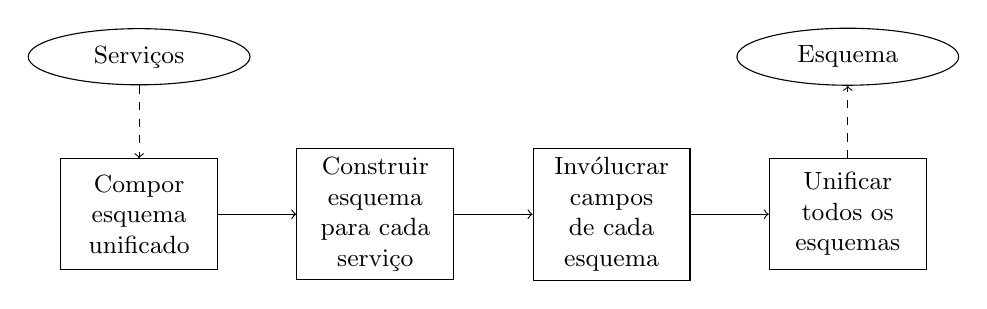
\begin{tikzpicture}[font=\small,text width=5em, text centered]
    \node [rectangle,draw,minimum height=4em] (composeSchema) {Compor esquema unificado};
    \node [ellipse,draw,draw, above of=composeSchema,node distance=2cm] (services) {Serviços};
    \node [rectangle,draw,minimum height=4em, right of=composeSchema,node distance=3cm] (buildSchema) {Construir esquema para cada serviço};
    \node [rectangle,draw,minimum height=4em, right of=buildSchema,node distance=3cm] (wrapSchema) {Invólucrar campos de cada esquema};
    \node [rectangle,draw,minimum height=4em, right of=wrapSchema,node distance=3cm] (deepExtendSchema) {Unificar todos os esquemas};
    \node [ellipse,draw, above of=deepExtendSchema,node distance=2cm] (schema) {Esquema};
    \draw [->] (composeSchema) -- (buildSchema);
    \draw [->] (buildSchema) -- (wrapSchema);
    \draw [->] (wrapSchema) -- (deepExtendSchema);
    \draw [->,dashed] (services) -- (composeSchema);
    \draw [->,dashed] (deepExtendSchema) -- (schema);
  \end{tikzpicture}
  \caption{Criação de esquema}
\end{figure}

O processo de criação de esquema começa resolvendo cada função de configuração de serviço e construindo um esquema GraphQL para cada um. Após, por razões de preferência de desenvolvimento, é feito o invólucro dos campos de cada esquema e para cada um estende-se até gerar um esquema unificado.

\begin{figure}[H]
  \centering
  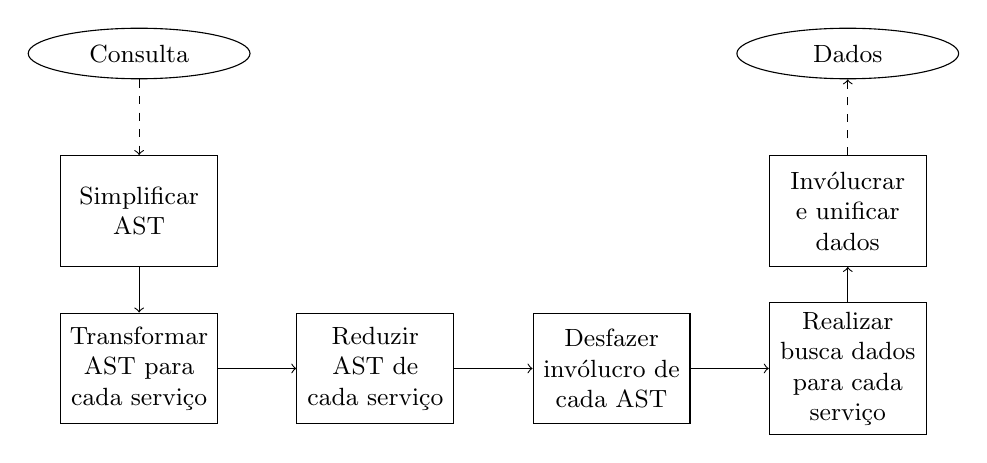
\begin{tikzpicture}[font=\small,text width=5em, text centered]
    \node [rectangle,draw,minimum height=4em] (simplifyAST) {Simplificar AST};
    \node [ellipse,draw, above of=simplifyAST,node distance=2cm] (services) {Consulta};
    \node [rectangle,draw,minimum height=4em, below of=simplifyAST,node distance=2cm] (transformAST) {Transformar AST para cada serviço};
    \node [rectangle,draw,minimum height=4em, right of=transformAST,node distance=3cm] (reduceASTs) {Reduzir AST de cada serviço};
    \node [rectangle,draw,minimum height=4em, right of=reduceASTs,node distance=3cm] (unwrapAST) {Desfazer invólucro de cada AST};
    \node [rectangle,draw,minimum height=4em, right of=unwrapAST,node distance=3cm] (fetchData) {Realizar busca dados para cada serviço};
    \node [rectangle,draw,minimum height=4em, above of=fetchData,node distance=2cm] (wrapData) {Invólucrar e unificar dados};
    \node [ellipse,draw, above of=wrapData,node distance=2cm] (schema) {Dados};
    \draw [->] (simplifyAST) -- (transformAST);
    \draw [->] (transformAST) -- (reduceASTs);
    \draw [->] (reduceASTs) -- (unwrapAST);
    \draw [->] (unwrapAST) -- (fetchData);
    \draw [->] (fetchData) -- (wrapData);
    \draw [->,dashed] (services) -- (simplifyAST);
    \draw [->,dashed] (wrapData) -- (schema);
  \end{tikzpicture}
  \caption{Consulta de dados}
\end{figure}

O processo de consulta de dados começa através de uma execução de consulta GraphQL. Primeiro é convertido a estrutura AST em um formato mais simplificado para se trabalhar. Após, transforma-se o AST principal em um AST especifico para cada serviço. Com as árvores de consulta, é feito a redução da árvore aplicando-se o algoritmo de busca. Após, é desfeito o invólucro de cada AST para poder realizar a busca de dados no serviço correspondente. Por fim, ao retornar os dados, realiza-se novamente o invólucro e estende-se cada dado até gerar um dado unificado.
\section{Implementação}

A partir do planejamento de projeto e especificação da ferramenta baseado no modelo proposto, foram implementados dez funções no total para testes em plataforma web. Quatro delas responsáveis por gerar o esquema, criando o intermediador. Três para analisar o AST das consultas e outras três para transformar o AST em requisições para API de cada serviço. Além disso, três dessas funções são extensíveis (substituíveis) através de adaptadores, sendo que apenas uma delas é pública.

A seguir, é descrito brevemente as 3 categorias de funções, junto com seu objetivo e a assinatura de cada método escrito em JavaScript. \\

\textbf{Funções para criação do esquema} \\

Representam quatro funções e seu principal objetivo é compor, de forma assíncrona, um esquema GraphQL unificado a partir das funcões de configuração de cada serviço. Sendo "composeSchema" a única função pública da ferramenta.

\begin{figure}[H]
  \centering
  \begin{minted}[frame=single,framesep=10pt,fontsize=\footnotesize]{text}
  function composeSchema(
    services: [Service]
  ): Promise<GraphQLSchema>

  function buildSchema(
    schema: JSON
  ): Promise<GraphQLSchema>

  function wrapSchema(
    schema: GraphQLSchema, 
    wrapper: Wrapper
  ): Promise<GraphQLSchema>

  function deepExtendSchema(
    schemas: [GraphQLSchema]
  ): Promise<GraphQLSchema>
  \end{minted}
  \caption{Assinatura das funções para criação do esquema}
\end{figure}

\textbf{Funções para análise de AST} \\

São três funções que buscam analisar o AST gerado por uma consulta GraphQL no esquema através de um algoritmo que simplifica, transforma e reduz em um AST específico e performático para cada serviço.

\begin{figure}[H]
  \centering
  \begin{minted}[frame=single,framesep=10pt,fontsize=\footnotesize]{text}
  function simplifyAST(
    value: AST, 
    info: JSON
  ): SimplifiedAST

  function transformAST(
    schema: JSON,
    clientSchema: GraphQLSchema, 
    ast: SimplifiedAST
  ): SimplifiedAST

  function reduceASTs(
    rootAST: SimplifiedAST, 
    asts: [SimplifiedAST]
  ): void
  \end{minted}
  \caption{Assinatura das funções para análise de AST}
\end{figure}

\textbf{Funções para busca de dados} \\

São as três últimas funções responsáveis por converter os ASTs retornados e realizar as respectivas requisições para a API de cada serviço em busca de dados.

\begin{figure}[H]
  \centering
  \begin{minted}[frame=single,framesep=10pt,fontsize=\footnotesize]{text}
  function unwrapAST(
    ast: SimplifiedAST, 
    schema: GraphQLSchema, 
    wrapper: Wrapper
  ): SimplifiedAST

  function fetchData(
    schema: JSON, 
    ast: SimplifiedAST, 
    url: string
  ): Promise<JSON>

  function wrapData(
    data: JSON, 
    schema: JSON, 
    wrapper: Wrapper
  ): Promise<JSON>
  \end{minted}
  \caption{Assinatura das funções para busca de dados}
\end{figure}

\section{Validação}

Com o objetivo de validar o modelo proposto através da ferramenta desenvolvida para plataforma web, é feito uma pesquisa comparativa focando o impacto do seu uso em relação à mudanças no fluxo de dados. Para isso será desenvolvido um ambiente de validação onde dois clientes, um com a ferramenta e o outro não, realizam três consultas na API de um serviço REST. Após, será aplicado uma série de mudanças no fluxo de dados da API REST e coletado os dados para análise do impacto causado no código de busca desses clientes. \\

\textbf{Escopo de serviço} \\

Foi escolhido trabalhar com um escopo de serviço SWAPI (Starwars), bastante utilizado para análise de implementações de tecnologias e estilos de arquitetura em diversas linguagens de programação. Nele, são descritos seis entidades (Pessoa, Filme, Espaçonave, Veículo, Espécie, Planeta) e seus respectivos relacionamentos. Na tabela 6, é descrito os pontos de acesso da API REST (SWAPI) utilizada na validação. Nota-se que o um nível de expansão refere-se a profundidade relacionamentos de dados JSON retornados pelo ponto de acesso.

\begin{table}[H]
  \centering
  \begin{tabular}{|l|c|c|}
    \hline
    URI & Descrição & Nível de expansão \\
    \hline
    /people & Busca lista de pessoas & 0 \\
    \hline
    /people/:id & Busca pessoa pelo id & 0 \\
    \hline
    /films & Busca lista de filmes & 0 \\
    \hline
    /films/:id & Busca filme pelo id & 0 \\
    \hline
    /starships & Busca lista de espaçonaves & 0 \\
    \hline
    /starships/:id & Busca espaçonave pelo id & 0 \\
    \hline
    /vehicles & Busca lista de veículos & 0 \\
    \hline
    /vehicles/:id & Busca veículo pelo id & 0 \\
    \hline
    /species & Busca lista de espécies & 0 \\
    \hline
    /species/:id & Busca espécie pelo id & 0 \\
    \hline
    /planets & Busca lista de planetas & 0 \\
    \hline
    /planets/:id & Busca planeta pelo id & 0 \\
    \hline
  \end{tabular}
  \caption{Pontos de acesso SWAPI para busca de dados}
\end{table}

\textbf{Perguntas e respostas esperadas} \\

Com o propósito de explorar cada ponto de acesso para busca de dados na SWAPI, foram pensadas em três perguntas de média complexidade e onde fossem envolvidos ao menos três das entidades para consulta na API. Para cada pergunta existe apenas uma resposta certa, onde sua lógica é baseada em campos das estruturas de dados de retorno nos pontos de acesso.

\begin{enumerate}
\item[\textbf{Q1.}] Qual o nome do filme no qual aparece mais personagens oriundos de um planeta deserto? \textbf{R:} "Revenge of the Sith"
\item[\textbf{Q2.}] Qual o nome da espécie predominante entre os habitantes do planeta "Tatooine"? \textbf{R:} "Droid"
\item[\textbf{Q3.}] Qual o nome do personagem que mais pilota espaçonaves e veículos durante o filme "A New Hope"? \textbf{R:} "Chewbacca" \\
\end{enumerate}

Falar sobre como é feito o fluxo de dados para acesso das informações.

\begin{table}[H]
  \centering
  \begin{tabular}{|c|c|c|}
    \hline
    Pergunta & Fluxo de Dados & Número de requisições \\
    \hline
    Q1 & \begin{minipage}[t]{0.4\textwidth}
      \begin{itemize}
        \item[\textbf{GET}] /api/films
        \item[\textbf{GET}] /api/people/:id
        \item[\textbf{GET}] /api/planet/:id
      \end{itemize}
    \end{minipage} & \begin{minipage}[t]{0.4\textwidth}
      \begin{itemize}
        \item[\textbf{x1}] films
        \item[\textbf{xN}] films.characters
        \item[\textbf{xN}] films.characters.homeworld
      \end{itemize}
    \end{minipage} \\
    \hline
    Q2 & \begin{minipage}[t]{0.4\textwidth}
      \begin{itemize}
        \item[\textbf{GET}] /api/planets/1
        \item[\textbf{GET}] /api/people/:id
        \item[\textbf{GET}] /api/species/:id
      \end{itemize}
    \end{minipage} & \begin{minipage}[t]{0.4\textwidth}
      \begin{itemize}
        \item[\textbf{x1}] planet
        \item[\textbf{xN}] planet.residents
        \item[\textbf{xN}] planet.residents.species
      \end{itemize}
    \end{minipage} \\
    \hline
    Q3 & \begin{minipage}[t]{0.4\textwidth}
      \begin{itemize}
        \item[\textbf{GET}] /api/films/1
        \item[\textbf{GET}] /api/starships/:id
        \item[\textbf{GET}] /api/people/:id
        \item[\textbf{GET}] /api/vehicles/:id
        \item[\textbf{GET}] /api/people/:id
      \end{itemize}
    \end{minipage} & \begin{minipage}[t]{0.4\textwidth}
      \begin{itemize}
        \item[\textbf{x1}] film
        \item[\textbf{xN}] film.starships
        \item[\textbf{xN}] film.starships.pilots
        \item[\textbf{xN}] film.vehicles
        \item[\textbf{xN}] film.vehicles.pilots
      \end{itemize}
    \end{minipage} \\
    \hline
  \end{tabular}
  \caption{Fluxo de dados para responder as perguntas}
\end{table}

\textbf{Mudanças no fluxo de dados} \\

É proposto quatro tipos de mudanças no fluxo de dados para quebra de contrato, onde cada mudança testa a capacidade da ferramenta em a adaptar a comunicação através da atualização dos metadados do serviço. \\

\begin{enumerate}
\item[\textbf{C1.}] Mudança no endereço de ponto de acesso.
\item[\textbf{C2.}] Mudança no nível de estrutura de resposta.
\item[\textbf{C3.}] Adição de ponto de acesso otimizado.
\item[\textbf{C4.}] Remoção de ponto de acesso deprecado.
\end{enumerate}

Falar sobre as alterações no fluxo de dados mais em detalhe.

\begin{table}[H]
  \centering
  \begin{tabular}{|c|c|c|}
    \hline
    Mudança & Descrição & Questões afetadas \\
    \hline
  \end{tabular}
  \caption{Changelog das alterações no fluxo de dados}
\end{table}

% c1
% - URI /films renamed to /movies. \\
% - URI /films/:id renamed to /movies/:id

% c2
% - pilots field from URI /starships/:id expanded. \\
% - pilots field from URI /vehicles/:id expanded.

% c3
% - URI /tatooine added. \\
% - URI /films/:id/characters added.

% c4
% - URI /planet/:id removed. \\
% - URI /people/:id/homeworld added.

\textbf{Variáveis} \\

É descrito cinco variáveis para análise dos testes de validação. Todos são quantitativas e coletadas no cliente após cada processo de mudança da API. Totalizando um número de 20 dados possíveis para análise no final de sua execução.

\begin{table}[H]
  \centering
  \begin{tabular}{|c|c|c|}
    \hline
    Variável & Unidade & Tipo \\
    \hline
    Porcentagem de acerto & \% & Quantitativa \\
    \hline
    Tamanho de resposta & kb & Quantitativa \\
    \hline
    Número de requisições & inteiro & Quantitativa \\
    \hline
    Tempo de busca de metadados & ms & Quantitativa \\
    \hline
    Tempo de processamento & ms & Quantitativa \\
    \hline
  \end{tabular}
  \caption{Variáveis de coleta e análise}
\end{table}

 
 
 
 
 
 

 


\chapter{Validação}

Com o objetivo de validar o modelo proposto, é realizada uma pesquisa comparativa com foco no impacto da relação do uso da ferramenta implementada e mudanças no fluxo de dados sobre APIs Web. Para isso, é desenvolvido um ambiente de validação onde dois clientes, um com a ferramenta e o outro não, realizam três consultas de dados sobre uma API REST. Por fim, é aplicada uma série de quatro mudanças no fluxo de dados da API e coletados os dados para análise do impacto causado no código de busca desses clientes. \\

\textbf{Escopo de serviço} \\

Escolheu-se trabalhar com um escopo de serviço conhecido como SWAPI (\textit{Starwars API}), bastante utilizado para análise de implementações de tecnologias e estilos de arquitetura em linguagens de programação. Nele, são descritas seis entidades (Pessoa, Filme, Espaçonave, Veículo, Espécie, Planeta) e seus respectivos relacionamentos. Dentro do escopo de serviço, é implementada uma API REST que expõe consultas dessas entidades em formato de representação JSON através de URIs, listadas na tabela 5. Nota-se que as representações possuem apenas um nível de expansão, ou seja, para acesso aos relacionamentos é preciso consultar a API através de links descritos pela estrutura de retorno.

\begin{table}[H]
  \centering
  \begin{tabular}{|l|c|}
    \hline
    URI & Descrição \\
    \hline
    /people & Busca lista de pessoas \\
    \hline
    /people/:id & Busca pessoa pelo id \\
    \hline
    /films & Busca lista de filmes \\
    \hline
    /films/:id & Busca filme pelo id \\
    \hline
    /starships & Busca lista de espaçonaves \\
    \hline
    /starships/:id & Busca espaçonave pelo id \\
    \hline
    /vehicles & Busca lista de veículos \\
    \hline
    /vehicles/:id & Busca veículo pelo id \\
    \hline
    /species & Busca lista de espécies \\
    \hline
    /species/:id & Busca espécie pelo id \\
    \hline
    /planets & Busca lista de planetas \\
    \hline
    /planets/:id & Busca planeta pelo id \\
    \hline
  \end{tabular}
  \caption{Descrição das URIs SWAPI}
\end{table}

\textbf{Perguntas e respostas esperadas} \\

Com o propósito de explorar cada URI para consulta de dados na SWAPI, foram determinadas três perguntas onde fossem envolvidas pelo menos três das entidades do escopo. Para cada pergunta existe apenas uma resposta certa e sua lógica é baseada em campos das estruturas de dados de retorno.

\begin{enumerate}
\item[\textbf{Q1.}] Qual o nome do filme no qual aparecem mais personagens oriundos de um planeta deserto? \textbf{R:} "Revenge of the Sith"
\item[\textbf{Q2.}] Qual o nome da espécie predominante entre os habitantes do planeta "Tatooine"? \textbf{R:} "Droid"
\item[\textbf{Q3.}] Qual o nome do personagem que mais pilota espaçonaves e veículos durante o filme "A New Hope"? \textbf{R:} "Chewbacca"
\end{enumerate}

No intuito de atingir as respostas esperadas, a tabela 6 descreve o fluxo de dados necessário para responder cada pergunta através da consulta de dados na SWAPI.

\begin{table}[H]
  \centering
  \begin{tabular}{|c|c|c|}
    \hline
    Pergunta & Requisições & Número de chamadas \\
    \hline
    Q1 & \begin{minipage}[t]{0.3\textwidth}
      \begin{itemize}
        \item[\textbf{GET}] /api/films
        \item[\textbf{GET}] /api/people/:id
        \item[\textbf{GET}] /api/planet/:id
      \end{itemize}
    \end{minipage} & \begin{minipage}[t]{0.5\textwidth}
      \begin{itemize}
        \item[\textbf{x1}] films
        \item[\textbf{x162}] films.characters
        \item[\textbf{x162}] films.characters.homeworld
      \end{itemize}
    \end{minipage} \\
    \hline
    Q2 & \begin{minipage}[t]{0.3\textwidth}
      \begin{itemize}
        \item[\textbf{GET}] /api/planets/1
        \item[\textbf{GET}] /api/people/:id
        \item[\textbf{GET}] /api/species/:id
      \end{itemize}
    \end{minipage} & \begin{minipage}[t]{0.5\textwidth}
      \begin{itemize}
        \item[\textbf{x1}] planet
        \item[\textbf{x10}] planet.residents
        \item[\textbf{x2}] planet.residents.species
      \end{itemize}
    \end{minipage} \\
    \hline
    Q3 & \begin{minipage}[t]{0.3\textwidth}
      \begin{itemize}
        \item[\textbf{GET}] /api/films/1
        \item[\textbf{GET}] /api/starships/:id
        \item[\textbf{GET}] /api/people/:id
        \item[\textbf{GET}] /api/vehicles/:id
        \item[\textbf{GET}] /api/people/:id
      \end{itemize}
    \end{minipage} & \begin{minipage}[t]{0.5\textwidth}
      \begin{itemize}
        \item[\textbf{x1}] film
        \item[\textbf{x8}] film.starships
        \item[\textbf{x9}] film.starships.pilots
        \item[\textbf{x4}] film.vehicles
        \item[\textbf{x0}] film.vehicles.pilots
      \end{itemize}
    \end{minipage} \\
    \hline
  \end{tabular}
  \caption{Fluxo de dados para responder as perguntas}
\end{table}

\textbf{Consultas GraphQL e metadados} \\

Para permitir a comunicação entre o cliente que faz o uso da ferramenta com a SWAPI, foi preciso implementar três consultas GraphQL (uma para cada pergunta), além de descrever os metadados da API REST em formato JSON Hyper-Schema. Na figura 24, foram  selecionados apenas os campos necessários para o funcionamento da lógica de resposta. Em relação aos metadados da figura 25, foram descritas apenas as URIs utilizadas.

\begin{figure}[H]
  \centering
  \begin{minted}[frame=single,framesep=10pt,fontsize=\footnotesize]{text}
      query q1 {
        allFilms {
          title
          characters {
            homeworld {
              climate
            }
          }
        }
      }

      query q2 {
        planet(planetID: 1) {
          residents {
            species {
              name
            }
          }
        }
      }

      query q3 {
        film(filmID: 1) {
          starships {
            pilots {
              name
            }
          }
          vehicles {
            pilots {
              name
            }
          }
        }
      }
  \end{minted}
  \caption{Consultas GraphQL para as perguntas}
\end{figure}

\begin{figure}[H]
  \centering
  \begin{minted}[frame=single,framesep=10pt,fontsize=\footnotesize]{text}
    {
      "$schema": "http://json-schema.org/draft-04/hyper-schema#",
      "title": "swapi",
      "type": "object",
      "definitions": {
        "allFilms": { ... },
        "film": { ... },
        "people": { ... },
        "planet": { ... },
        "species": { ... },
        "starship": { ... },
        "vehicle": { ... }
      },
      "properties": {
        "allFilms": { "$ref": "#/definitions/allFilms" },
        "film": { "$ref": "#/definitions/film" },
        "people": { "$ref": "#/definitions/people" },
        "planet": { "$ref": "#/definitions/planet" },
        "species": { "$ref": "#/definitions/species" },
        "starship": { "$ref": "#/definitions/starship" }
      },
      "links": [{
        "rel": "allFilms",
        "href": "/films",
        "targetSchema": {
          "$ref": "#/definitions/allFilms"
        }
      }, {
        "rel": "film",
        "href": "/films/{filmID}",
        "schema": { ... },
        "targetSchema": {
          "$ref": "#/definitions/film"
        }
      }, {
        "rel": "planet",
        "href": "/planets/{planetID}",
        "schema": { ... },
        "targetSchema": {
          "$ref": "#/definitions/planet"
        }
      }]
    }
  \end{minted}
  \caption{JSON Hyper-Schema para SWAPI}
\end{figure}

\textbf{Mudanças no fluxo de dados} \\

Para avaliar o impacto no código em ambos clientes, são propostos quatro tipos de mudanças não acumulativas na especificação da API que afetam o fluxo de dados. Cada uma busca por em teste a capacidade da ferramenta em se adaptar e realizar a comunicação mesmo após a alteração no fluxo. Nota-se que, para cada mudança na API do serviço, é preciso a atualização de seus metadados para a correta operação da ferramenta. A tabela 7 descreve o \textit{changelog} das mudanças realizadas.

\begin{table}[H]
  \centering
  \begin{tabular}{|c|c|c|}
    \hline
    Mudança & Descrição & Changelog \\
    \hline
    C1 & \begin{minipage}[t]{0.3\textwidth}
      Mudança de acesso em endereços.
    \end{minipage} & \begin{minipage}[t]{0.5\textwidth}
      \begin{itemize}
        \item Renomeação da URI /films para /movies.
        \item Renomeação da URI /films/:id para /movies/:id
      \end{itemize}
    \end{minipage} \\
    \hline
    C2 & \begin{minipage}[t]{0.3\textwidth}
      Mudança no nível da estrutura de resposta em endereços.
    \end{minipage} & \begin{minipage}[t]{0.5\textwidth}
      \begin{itemize}
        \item Expansão do campo pilots da URI /starships/:id
        \item Expansão do campo pilots da URI /vehicles/:id
      \end{itemize}
    \end{minipage} \\
    \hline
    C3 & \begin{minipage}[t]{0.3\textwidth}
      Introdução de novos endereços.
    \end{minipage} & \begin{minipage}[t]{0.5\textwidth}
      \begin{itemize}
        \item[\textbf{+}] Adição da URI /tatooine.
        \item[\textbf{+}] Adição da URI /films/:id/characters.
      \end{itemize}
    \end{minipage} \\
    \hline
    C4 & \begin{minipage}[t]{0.3\textwidth}
      Substituição de endereço \textit{deprecated}.
    \end{minipage} & \begin{minipage}[t]{0.5\textwidth}
      \begin{itemize}
        \item[\textbf{+}] Adição da URI /people/:id/homeworld.
        \item[\textbf{$-$}] Remoção da URI /planet/:id.
      \end{itemize}
    \end{minipage} \\
    \hline
  \end{tabular}
  \caption{Changelog do novo fluxo de dados}
\end{table}

\textbf{Variáveis} \\

São descritas cinco variáveis para análise dos quatro testes de validação em cada um dos clientes. Todas são quantitativas e coletadas no cliente após cada processo de mudança da API. Dessa maneira, totalizam um número de 40 dados normalizados possíveis para análise no final da execução nos dois clientes.

\begin{table}[H]
  \centering
  \begin{tabular}{|c|c|c|}
    \hline
    Variável & Unidade & Tipo \\
    \hline
    Porcentagem de acerto & \% & Quantitativa \\
    \hline
    Tamanho de resposta & kb & Quantitativa \\
    \hline
    Número de requisições & inteiro & Quantitativa \\
    \hline
    Tempo de busca de metadados & ms & Quantitativa \\
    \hline
    Tempo de processamento & ms & Quantitativa \\
    \hline
  \end{tabular}
  \caption{Variáveis de coleta e análise}
\end{table}

\section{Resultados}

Os resultados obtidos nos testes de validação apresentam a média dos valores coletados após diversas execuções dos quatro testes de mudança de forma sequencial em uma máquina virtual. Tanto o serviço SWAPI como os clientes JavaScript foram executados no mesmo ambiente computacional, porém com conexão local de latência 10mb/s para simulação de um ambiente distribuído. Para a variável de processamento, foram utilizados valores que pudessem representar um dispositivo computacional de médio porte. (1 CPU de 2.4 GHz e 4gb de RAM)

Inicialmente, observa-se na figura 28 que o cliente 1 (sem o uso da ferramenta) não apresenta um bom índice de acerto das respostas. Dentre as quatro mudanças, obteve apenas 58\% de acerto, sendo a C3 a única mudança em que conseguiu responder certo todas pois não houve mudança nas URIs que estava utilizando. Um resultado esperado, significando que houve quebra de contrato e impacto negativo ao código de busca.

Em contrapartida, o cliente 2 (com o uso da ferramenta) apresenta um resultado no índice de acerto da figura 29 36.61\% superior ao cliente 1. Com um total de 91,5\% de acerto, apenas não completou com 100\% de acerto pois a mudança C4 não permitiu que fosse possível acessar todos os dados necessários para a responder da pergunta Q2. Isso representa que a ferramenta foi capaz, através do intermediador, de evitar a criação de contrato e causar impacto negativo ao código de busca.

Nota-se que ambos os clientes não apresentaram erros na resposta, ao invés acabam não respondendo pois ocorre exceções durante o código de busca ou lógica devido ao impacto das mudanças no fluxo de dados.

\begin{figure}[H]
  \centering
  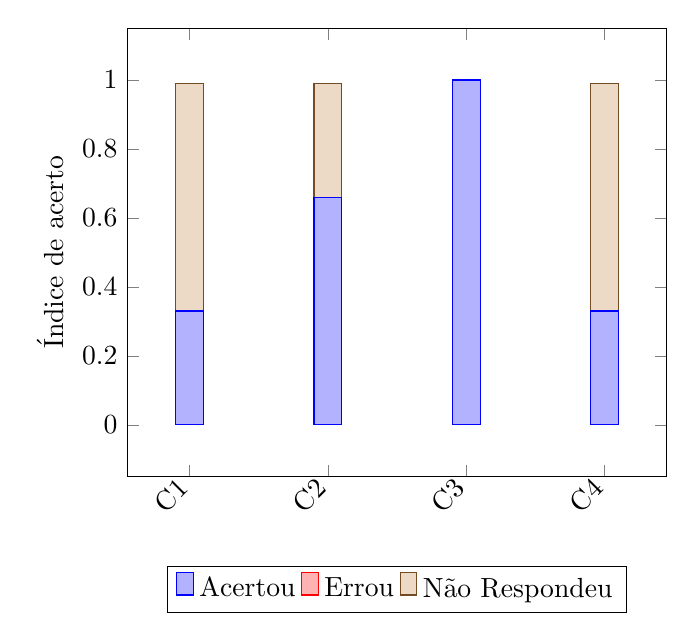
\begin{tikzpicture}
  \begin{axis}[
      ybar stacked,
      ymax=1,
      ymin=0,
      enlargelimits=0.15,
      legend style={at={(0.5,-0.20)},
        anchor=north,legend columns=-1},
      ylabel={Índice de acerto},
      symbolic x coords={C1, C2, C3, C4,
          C5, C6, C7},
      xtick=data,
      x tick label style={rotate=45,anchor=east},
      ]
  \addplot+[ybar] plot coordinates {(C1,0.33) (C2,0.66)
    (C3,1) (C4,0.33)};
  \addplot+[ybar] plot coordinates {(C1,0) (C2,0)
    (C3,0) (C4,0)};
  \addplot+[ybar] plot coordinates {(C1,0.66) (C2,0.33)
    (C3,0) (C4,0.66)};
  \legend{Acertou, Errou, Não Respondeu}
  \end{axis}
  \end{tikzpicture}
  \caption{Índice de acerto sem o uso da ferramenta}
\end{figure}

\begin{figure}[H]
  \centering
  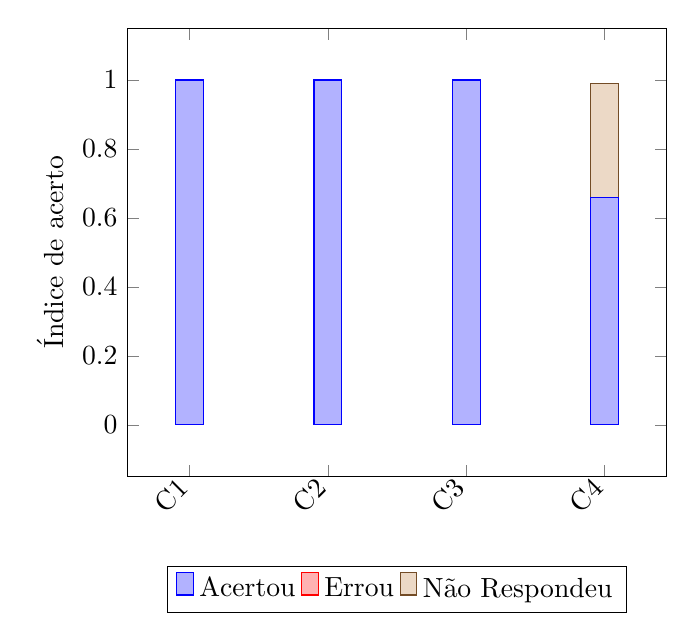
\begin{tikzpicture}
  \begin{axis}[
      ybar stacked,
      ymax=1,
      ymin=0,
      enlargelimits=0.15,
      legend style={at={(0.5,-0.20)},
        anchor=north,legend columns=-1},
      ylabel={Índice de acerto},
      symbolic x coords={C1, C2, C3, C4,
          C5, C6, C7},
      xtick=data,
      x tick label style={rotate=45,anchor=east},
      ]
  \addplot+[ybar] plot coordinates {(C1,1) (C2,1)
    (C3,1) (C4,0.66)};
  \addplot+[ybar] plot coordinates {(C1,0) (C2,0)
    (C3,0) (C4,0)};
  \addplot+[ybar] plot coordinates {(C1,0) (C2,0)
    (C3,0) (C4,0.33)};
  \legend{Acertou, Errou, Não Respondeu}
  \end{axis}
  \end{tikzpicture}
  \caption{Índice de acerto com o uso da ferramenta}
\end{figure}

Ao analisar a mudança C3 isoladamente, onde ambos conseguem responder com 100\% de acerto, percebe-se na figura 30 e 31 que o cliente 2 consegue realizar uma busca mais performática (menor número de requisição e tamanho de dados) que o cliente 1. Isso porque, após a mudança e sem alterar o código de busca de dados, a ferramenta consegue remapear as requisições geradas pelas consultas GraphQL graças ao algoritmo de implementação na automação das chamadas em URIs.

Outro ponto importante é que, após a mudança C3 e atualização dos metadados no cliente, o algoritmo da ferramenta percebe que há a possibilidade de realizar menos requisições em busca dos dados para responder as perguntas. O que resulta em uma redução de aproximadamente 54\% dos acessos entre o cliente 1 e cliente 2.

\begin{figure}[H]
  \centering
  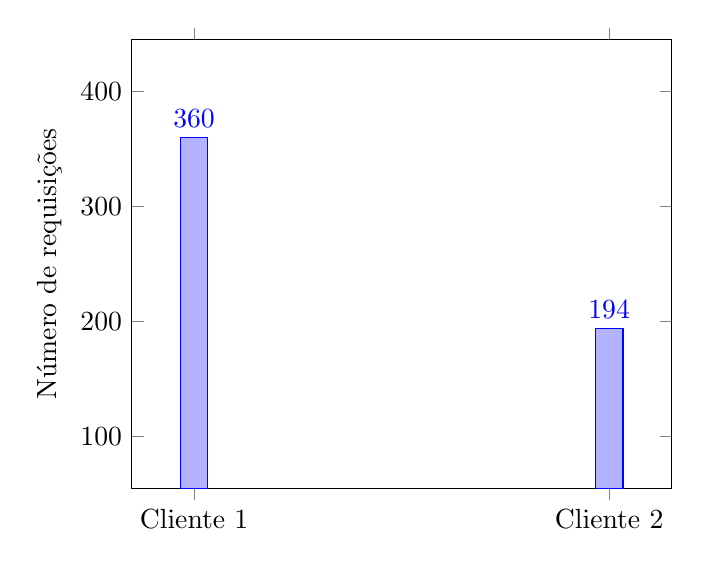
\begin{tikzpicture}
  \begin{axis}[
      ybar,
      ymax=400,
      ymin=100,
      enlargelimits=0.15,
      ylabel={Número de requisições},
      symbolic x coords={Cliente 1,Cliente 2},
      xtick=data,
      nodes near coords,
      nodes near coords align={vertical},
      ]
  \addplot coordinates {(Cliente 1,360) (Cliente 2,194)};
  \end{axis}
  \end{tikzpicture}
  \caption{Comparação no número de requisições C3}
\end{figure}

\begin{figure}[H]
  \centering
  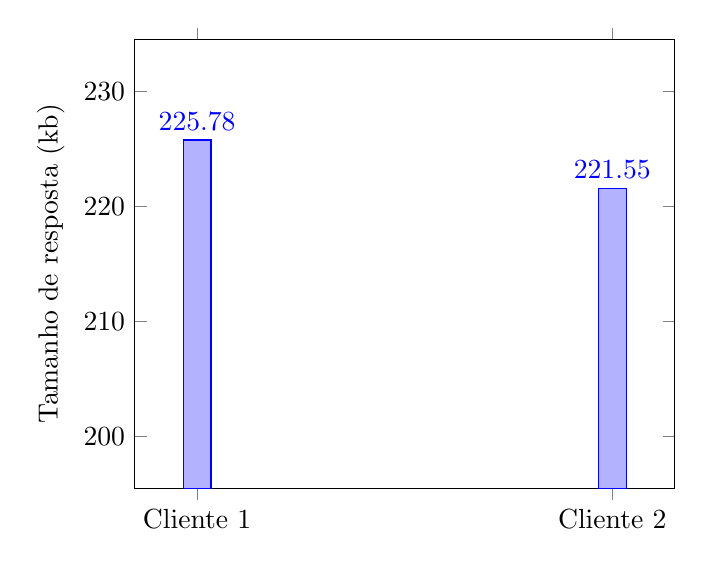
\begin{tikzpicture}
  \begin{axis}[
      ybar,
      ymax=230,
      ymin=200,
      enlargelimits=0.15,
      ylabel={Tamanho de resposta (kb)},
      symbolic x coords={Cliente 1,Cliente 2},
      xtick=data,
      nodes near coords,
      nodes near coords align={vertical},
      ]
  \addplot coordinates {(Cliente 1,225.777) (Cliente 2,221.547)};
  \end{axis}
  \end{tikzpicture}
  \caption{Comparação no tamanho de resposta C3}
\end{figure}

Apesar dos ganhos de performance e desenvolvimento através do uso da ferramenta vistos anteriormente, percebe-se na figura 32 um outro cenário em que indica o lado negativo do seu uso causado pelo tempo de \textit{overhead}\footnote{
  Processamento em excesso
}. Em média, a ferramenta atrasou em 1.7 segundos a execução na consulta de dados do cliente, sendo o tempo de busca de metadados responsável por somar mais da metade deste atraso inicial.

Contudo, é importante levar em conta que este tempo de \textit{overhead} é um impasse da ferramenta, mas também relativo ao tempo de vida do cliente que está sendo executado. Por exemplo, em clientes com tempo de vida curto ou que dependem de carregamento rápido, a ferramenta pode não ser a solução ideal. Nos demais casos, é visível os benefícios que seu uso pode trazer.

\begin{figure}[H]
  \centering
  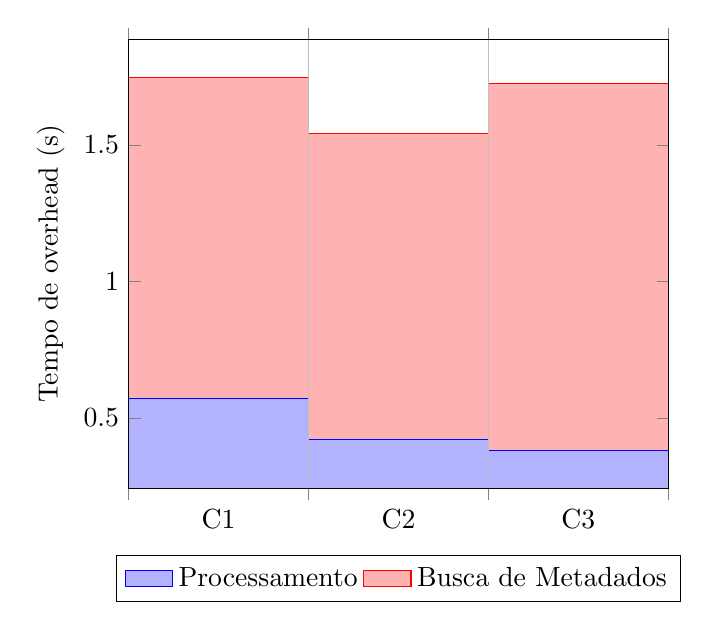
\begin{tikzpicture}
	\begin{axis}[
        ybar interval,
        ylabel={Tempo de overhead (s)},
        legend style={at={(0.5,-0.15)},
        anchor=north,legend columns=-1},
        const plot,
		stack plots=y,
		area style,
        symbolic x coords={C1,C2,C3,C4},
		enlarge x limits=false]
	\addplot coordinates
		{(C1,0.57) (C2,0.42) (C3,0.38) (C4,0.48)}
		\closedcycle;
	\addplot coordinates
		{(C1,1.178) (C2,1.123) (C3,1.343) (C4,1.185)}
		\closedcycle;
    \legend{Processamento,Busca de Metadados}
	\end{axis}
  \end{tikzpicture}
  \caption{Overhead da ferramenta}
\end{figure}


\chapter{Conclusão}

Tornou-se evidente através deste trabalho a vulnerabilidade do atual modelo de comunicação cliente-servidor em relação à possíveis mudanças no fluxo de dados ocorridas ao longo do tempo em APIs Web. Isso porque, com o aumento no número de serviços e diversidade de clientes distribuídos, existe uma necessidade em satisfazer a demanda de dados por clientes sem causar dependência e criação de contratos de acesso.

O esforço dedicado neste trabalho em resolver esta vulnerabilidade resultou na proposta de um novo modelo de comunicação possível de ser aplicado. Serviços que hesitam realizar mudanças no fluxo de dados devido à quebra de contrato, apresentam agora uma opção de evitar sua criação através da descrição dos metadados de sua API e o uso da ferramenta proposta para a busca de dados em seus clientes.

Além disso, uma das principais contribuição deste trabalho foi em mostrar os benefícios da busca de dados automatizada e a facilidade na composição de serviços que a ferramenta proporciona em clientes. Em seguida, mostrar a importância de escrever código de busca através de expressões como consultas GraphQL, ao invés de chamadas diretas em pontos de acesso de uma API.

Por fim, o trabalho é um exemplo de oportunidade concretizada graças ao uso formatos para descrição de APIs Web.

\section[Trabalhos Futuros]{Trabalhos Futuros}

\begin{itemize}
  \item Realização de testes de validação para a composição de serviços.
  \item Criação de novos adaptadores da ferramenta para formatos de descrição de APIs. (OpenAPI, RAML, API Blueprint)
  \item Implementação da especificação da ferramenta em outras plataformas de desenvolvimento. (Mobile, Desktop, etc)
  \item Aprimoramento do algoritmo de análise de consultas.
\end{itemize}

\begin{itemize}
\item Realizar mais testes de validação como a de composição de serviços, transição entre versões de API e estilos de arquitetura.
\item Criar novos adaptadores para formatos de descrição de APIs. (OpenAPI, RAML, API Blueprint)
\item Implementar a especificação da ferramenta em outras plataformas de desenvolvimento. (Android e iOS)
\item Melhorar o algoritmo de análise de consultas AST.
\end{itemize}


\bibliography{bibliografia/index}
\postextual
\begin{anexosenv}
  \chapter*{Funções da Ferramenta}
\input{pos-textual/anexo/funcoes-da-ferramenta/compose-schema}
\input{pos-textual/anexo/funcoes-da-ferramenta/build-schema}
\input{pos-textual/anexo/funcoes-da-ferramenta/wrap-schema}
\input{pos-textual/anexo/funcoes-da-ferramenta/deep-extend-schema}
\input{pos-textual/anexo/funcoes-da-ferramenta/simplify-ast}
\input{pos-textual/anexo/funcoes-da-ferramenta/transform-ast}
\input{pos-textual/anexo/funcoes-da-ferramenta/reduce-asts}
\input{pos-textual/anexo/funcoes-da-ferramenta/unwrap-ast}
\input{pos-textual/anexo/funcoes-da-ferramenta/fetch-data}
\input{pos-textual/anexo/funcoes-da-ferramenta/wrap-data}
\input{pos-textual/anexo/funcoes-da-ferramenta/deep-extend-data}

\chapter*{Funções do Adaptador}
\input{pos-textual/anexo/funcoes-do-adaptador/build-schema}
\input{pos-textual/anexo/funcoes-do-adaptador/transform-ast}
\input{pos-textual/anexo/funcoes-do-adaptador/fetch-data}

  
\end{anexosenv}

\end{document}
